%%%%%  Decoder %%%%%
\subsection{Reconstruction Quality Evaluation}

Our implementation of the Universal Style Transfer is adapted to use two different sets of encoder-decoder models: the models we trained according to section \ref{subsec:Models} (our), and the models offered to download by Li et al in their GitHub (reference). This means we can test \textbf{our implementation} of the UST algorithm with both sets of models. In this section we want to evaluate our models in comparison to the references in terms of image reconstruction, in order to asses the quality of our models training.

\subsubsection{Quantative Reconstruction Loss}
In order to quantify the reconstruction distortion induced by our trained models, in comparison to that of the reference models, we encode and then decode 1k content images from the COCO dataset using all 5 encoder-decoder pairs, and measure the pixel MSE and feature MSE. The pixel MSE measures the mean square error between the reconstructed image, $\hat{x}$, and the original one, $x$, i.e. $MSE(x - \hat{x})$. The feature MSE measures the error between the deep features of the reconstructed image and the original one. It is measured by again encoding $x$ and $\hat{x}$ and calculating $MSE(E(x)-E(\hat{x}))$. Table ~\ref{Tab:loss} displays the pixel loss (feature loss) per model, which are defined to be the average pixel MSE (feature MSE) over the 1k images.

% ecoder-decoder table %

\begin{center}
	\captionof{table}{Pixel and Feature Loss Per Model\label{Tab:loss}}
	\centering
	\begin{tabular}{ |>{\centering}p{2.5cm}||>{\centering}p{2.5cm}|>{\centering}p{2.5cm}|>{\centering}p{2.5cm}|>{\centering}p{2.5cm}| }
		\hline
		\multicolumn{5}{|c|}{\hspace{1.4cm} Pixel loss[$1\mathrm{e}{-4}$] \hspace{3cm}$\mid$ \hspace{1cm} Feature loss[$1\mathrm{e}{-2}$]} \\
		\hline
		architecture &Reference &Our &Reference &Our \tabularnewline
		\hline
		1 &$8.246$  &$802$   &$2.161$ &$0.7$\tabularnewline
		\hline
		2 &$2.374$  &$810$   &$1.257$ &$15.30$\tabularnewline
		\hline
		3 &$7.994$  &$884$   &$16.38$ &$86.60$\tabularnewline
		\hline
		4 &$0.281$  &$830$   &$25.09$ &$223.6$\tabularnewline
		\hline
		5 &$..$  &$..$   &$..$ &..\tabularnewline
		\hline
	\end{tabular}\\
\end{center}

\subsubsection{Qualitative Reconstruction Loss}
To demonstrate the image reconstruction performance of our trained models, we choose 5 different images and feed them as input to our encoder-decoder architectures, as well as to the reference architectures. The results, as presented in figure ~\ref{fig:reconstruction}, visualize the image reconstruction quality of our models in comparison to that of the references.\newline
In figure ~\ref{fig:reconstruction} (a) we present Our reconstruction which means the use of trained decoders as in VGG-19 \cite{bib20} and encoder, based on torchvision package.
As can be visually seen, our reconstruction images are less good than Li et al. \cite{bib11} results. Our results suffer from artifacts such as blurring and over smoothing, especially in small details such as faces. This artifacts are outcome of our trained decoder.

\begin{figure}[H]
	% first line
	\centering
	\begin{subfigure}[b]{0.13\linewidth}
		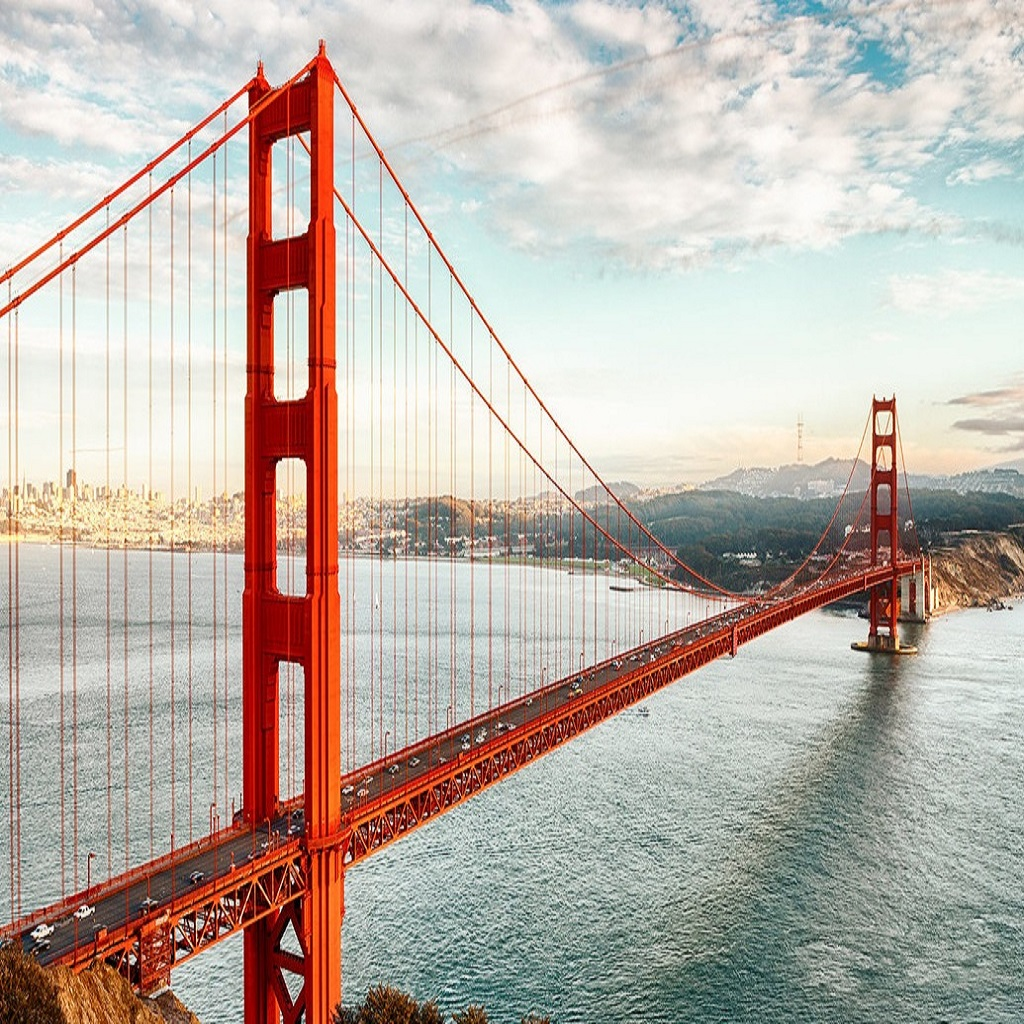
\includegraphics[width=\linewidth]{bridge_sq.jpg} % original num.1	
	\end{subfigure}
	\begin{subfigure}[b]{0.13\linewidth}
		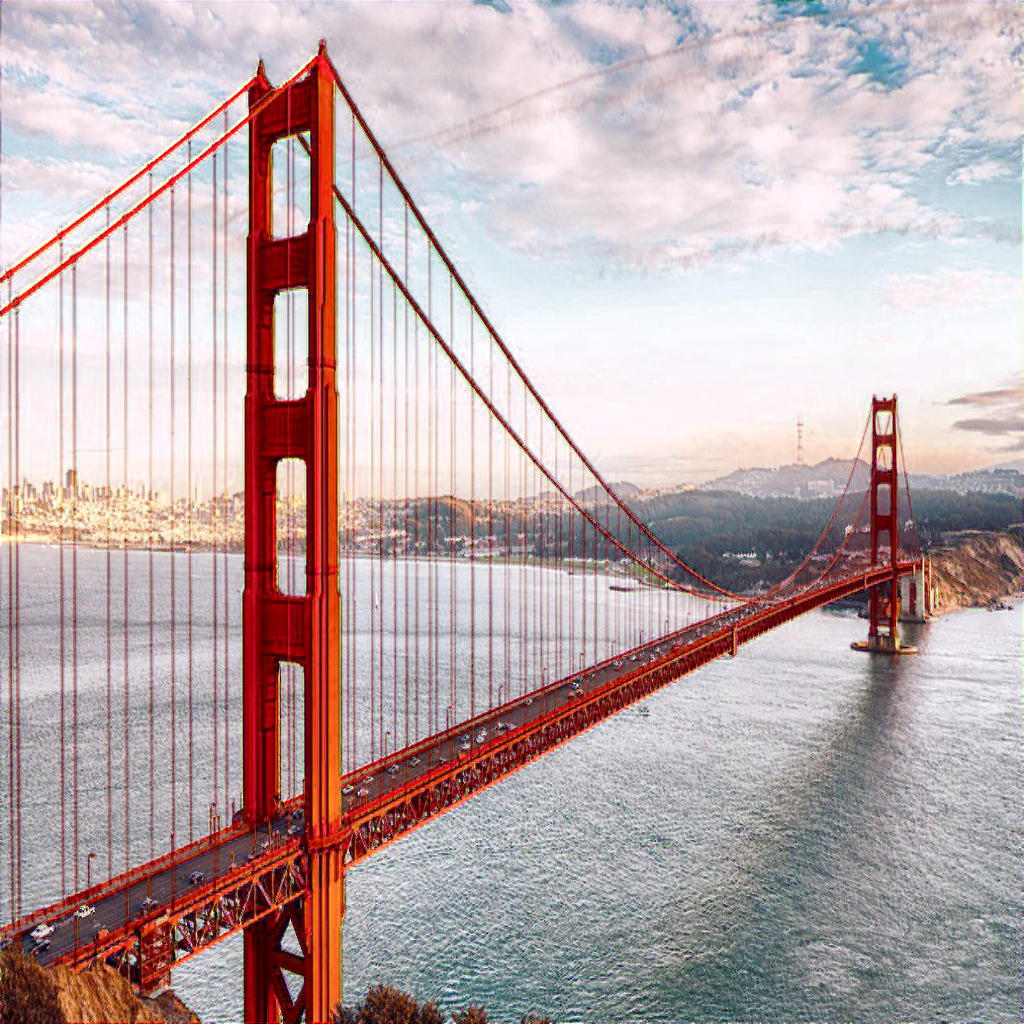
\includegraphics[width=\linewidth]{reconst_exper/dec_bridge_my_1_test.png} % our reconstruction arc1 num.1	
	\end{subfigure}
	\begin{subfigure}[b]{0.13\linewidth}
		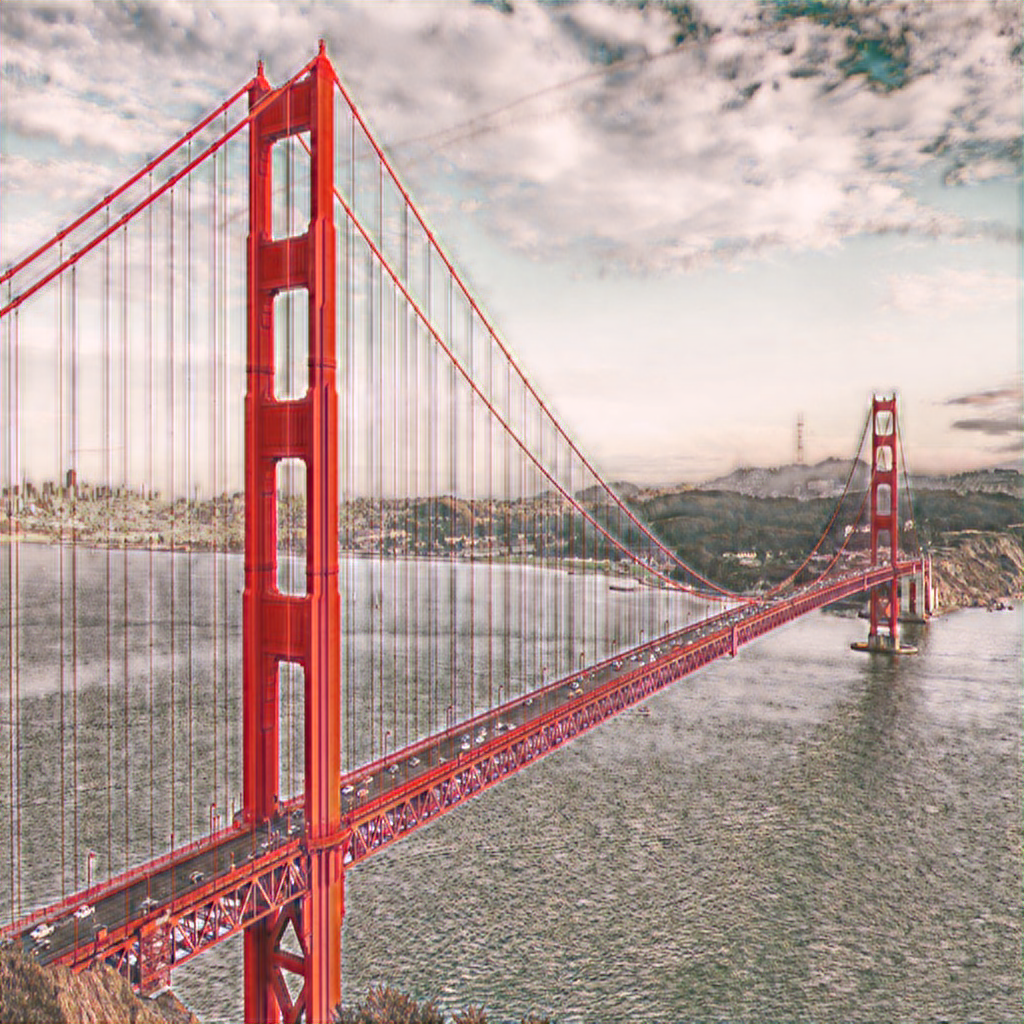
\includegraphics[width=\linewidth]{reconst_exper/dec_bridge_my_2_test.png} % our reconstruction arc2 num.1	
	\end{subfigure}
	\begin{subfigure}[b]{0.13\linewidth}
		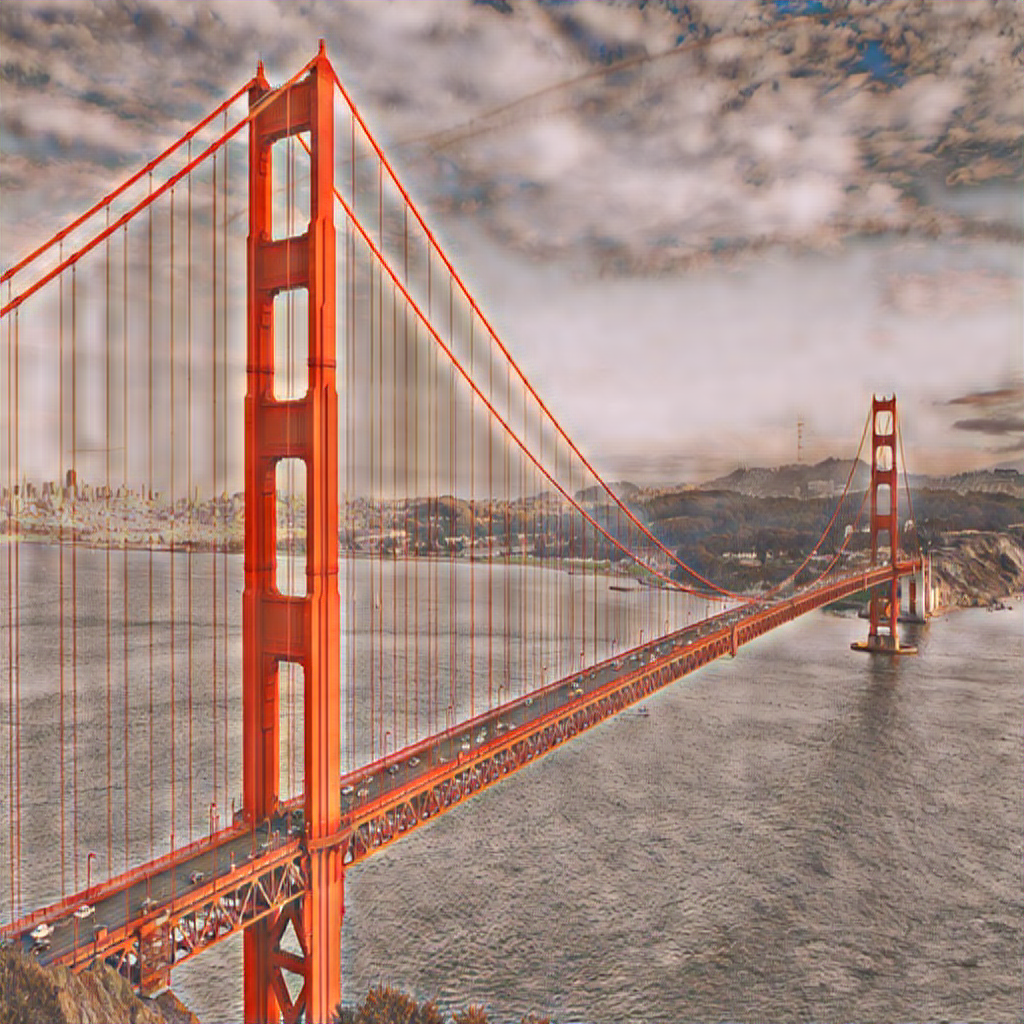
\includegraphics[width=\linewidth]{reconst_exper/dec_bridge_my_3_test.png} % our reconstruction arc3 num.1	
	\end{subfigure}
	\begin{subfigure}[b]{0.13\linewidth}
		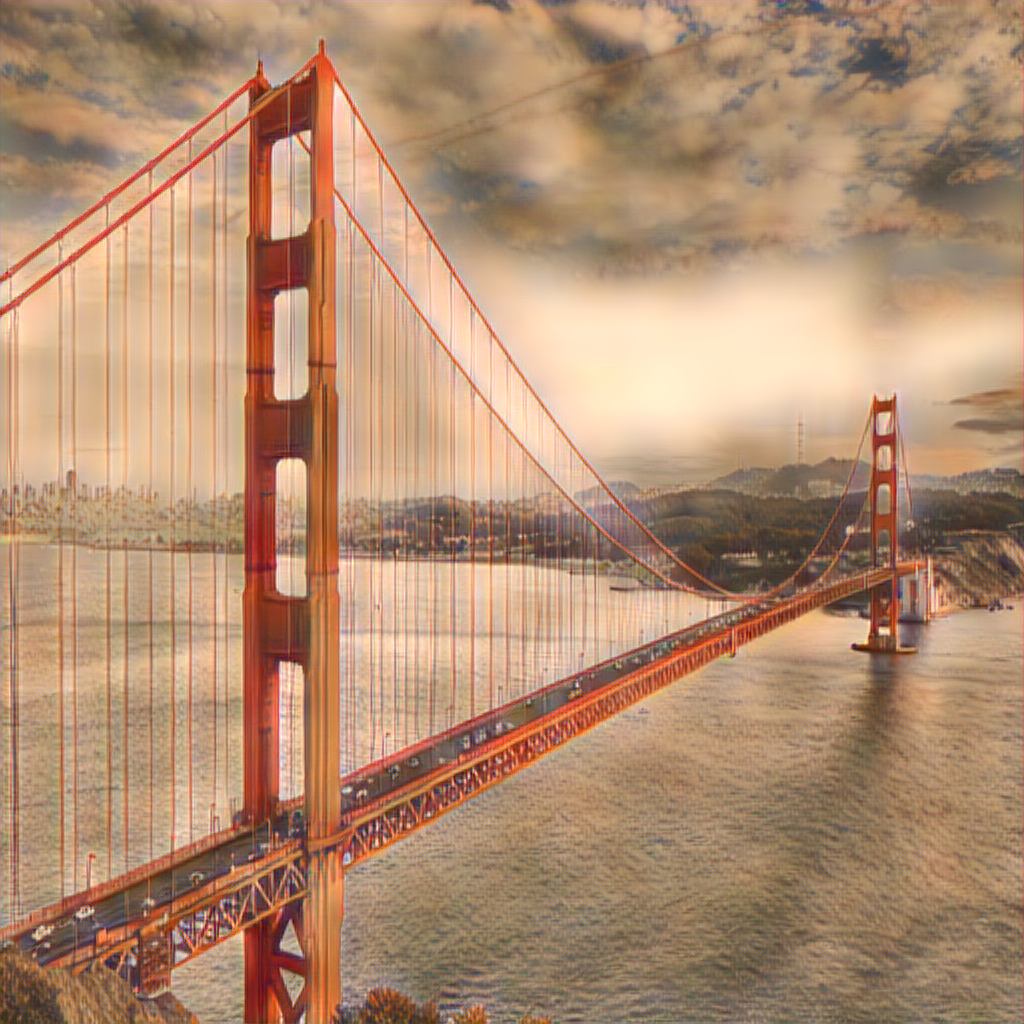
\includegraphics[width=\linewidth]{reconst_exper/dec_bridge_my_4_test.png} % our reconstruction arc4 num.1	
	\end{subfigure}
	\begin{subfigure}[b]{0.13\linewidth}
		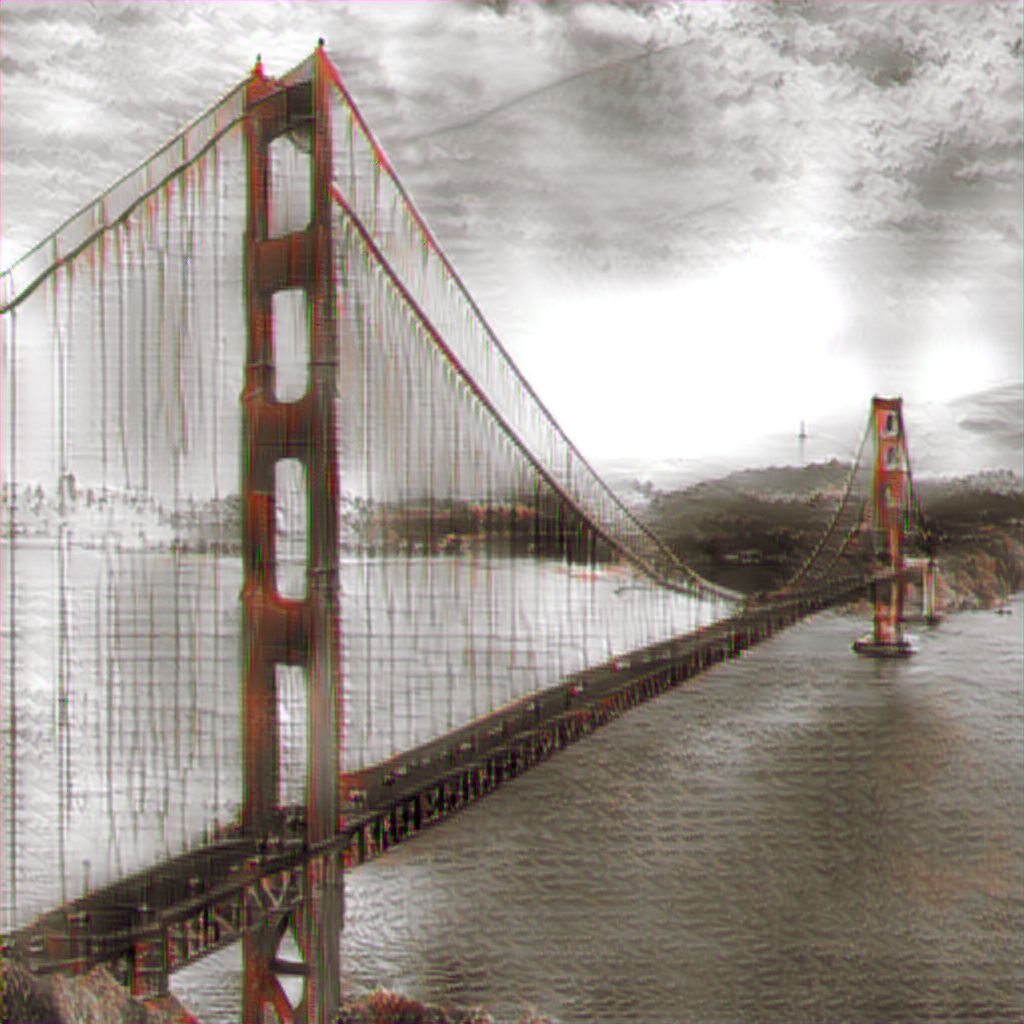
\includegraphics[width=\linewidth]{reconst_exper/dec_bridge_my_5_test.png} % our reconstruction arc5 num.1	
	\end{subfigure}
	\begin{subfigure}[b]{0.13\linewidth}
		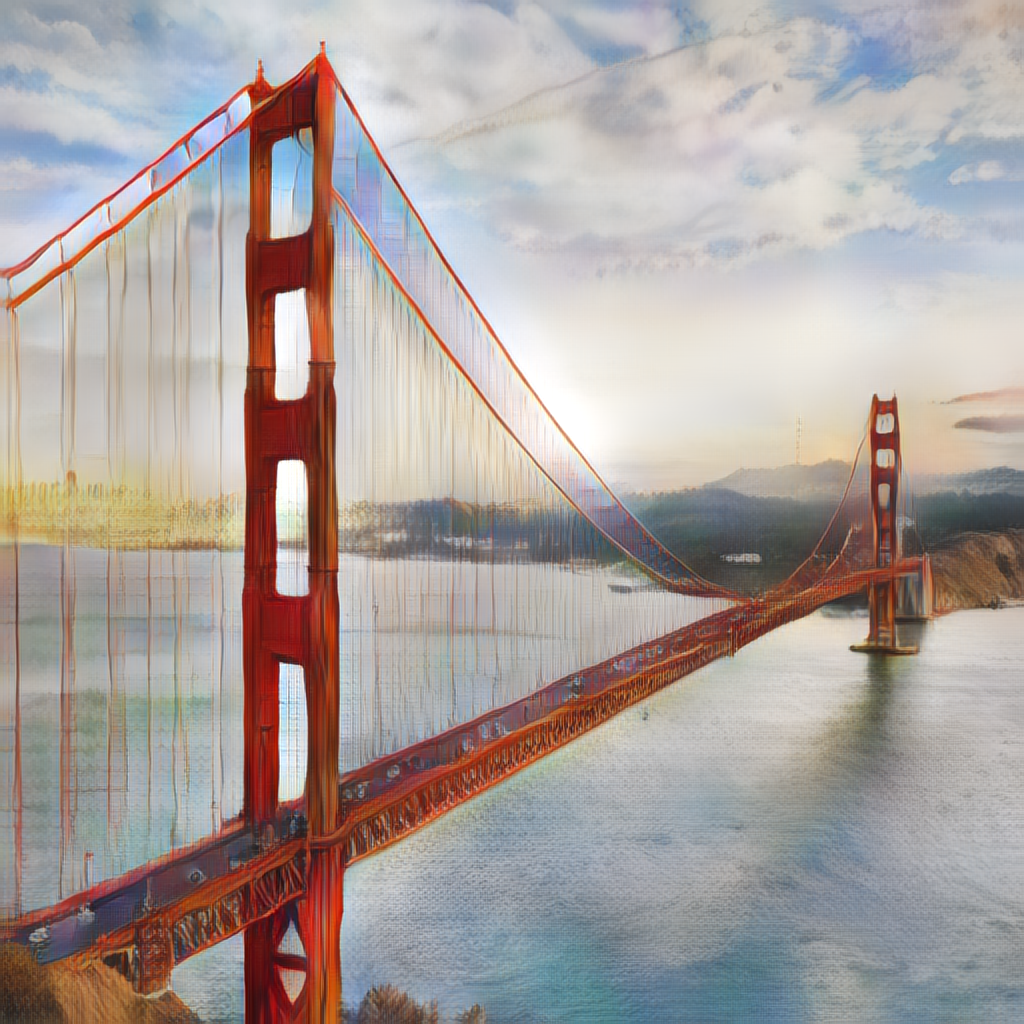
\includegraphics[width=\linewidth]{reconst_exper/dec_bridge_ref_5_test.png} % their reconstruction arc5 num.1	
	\end{subfigure}
	% second line
	\centering
	\begin{subfigure}[b]{0.13\linewidth}
		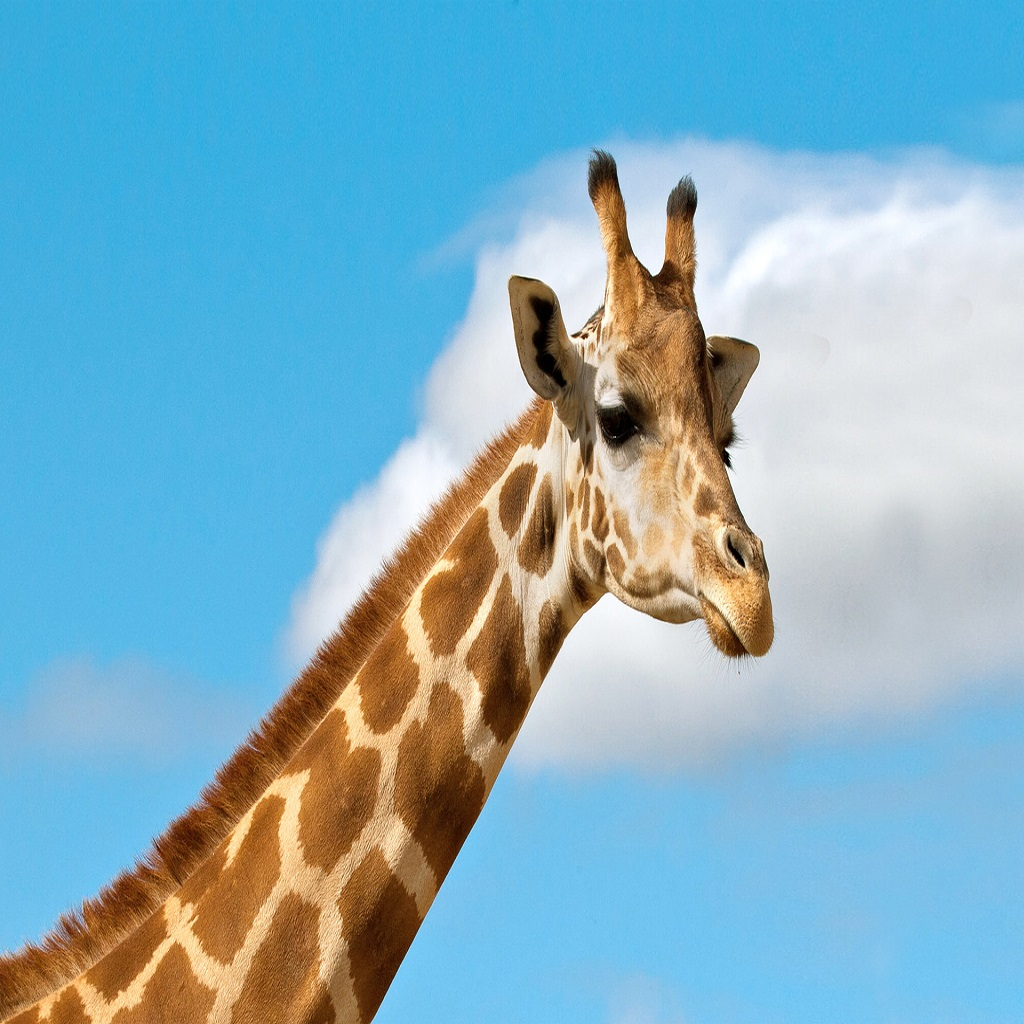
\includegraphics[width=\linewidth]{giraffe_sq.jpg} % original num.1	
	\end{subfigure}
	\begin{subfigure}[b]{0.13\linewidth}
		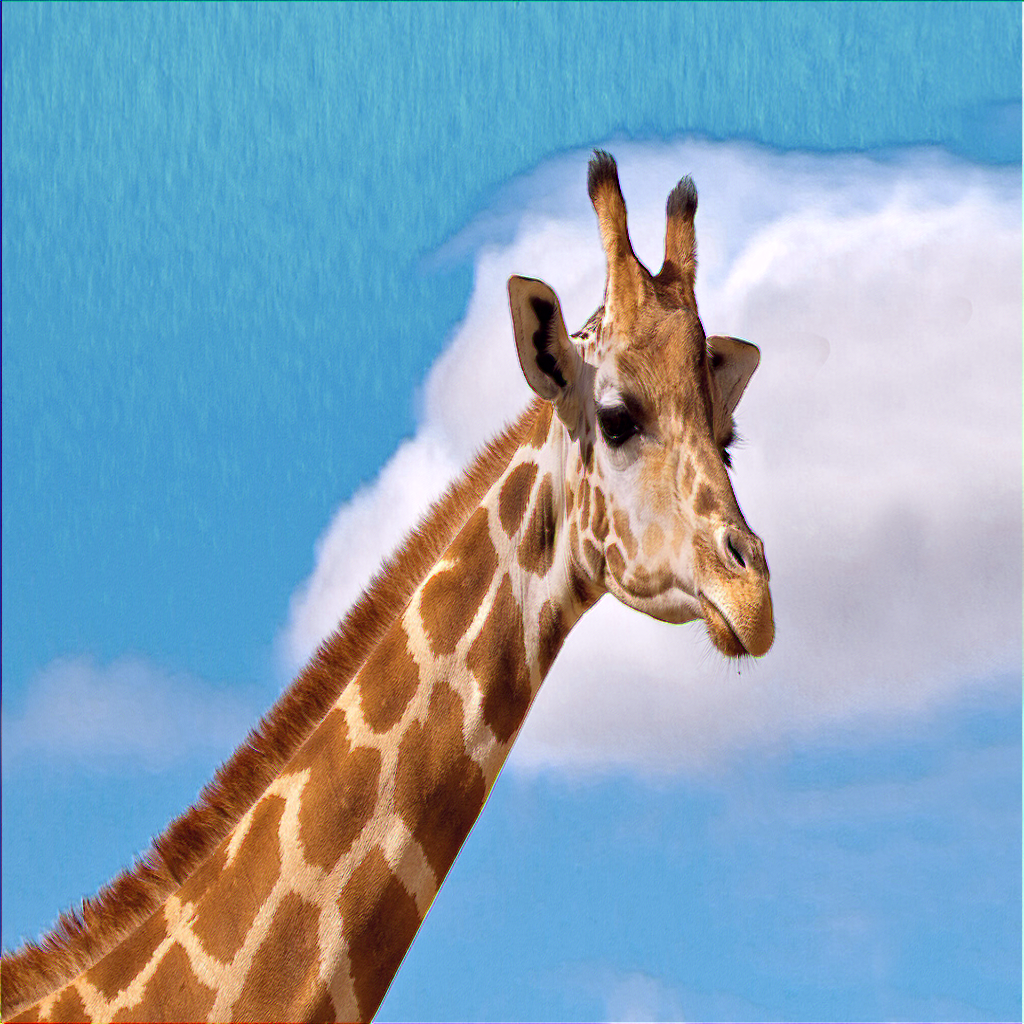
\includegraphics[width=\linewidth]{reconst_exper/dec_giraffe_my_1_test.png} % our reconstruction arc1 num.1	
	\end{subfigure}
	\begin{subfigure}[b]{0.13\linewidth}
		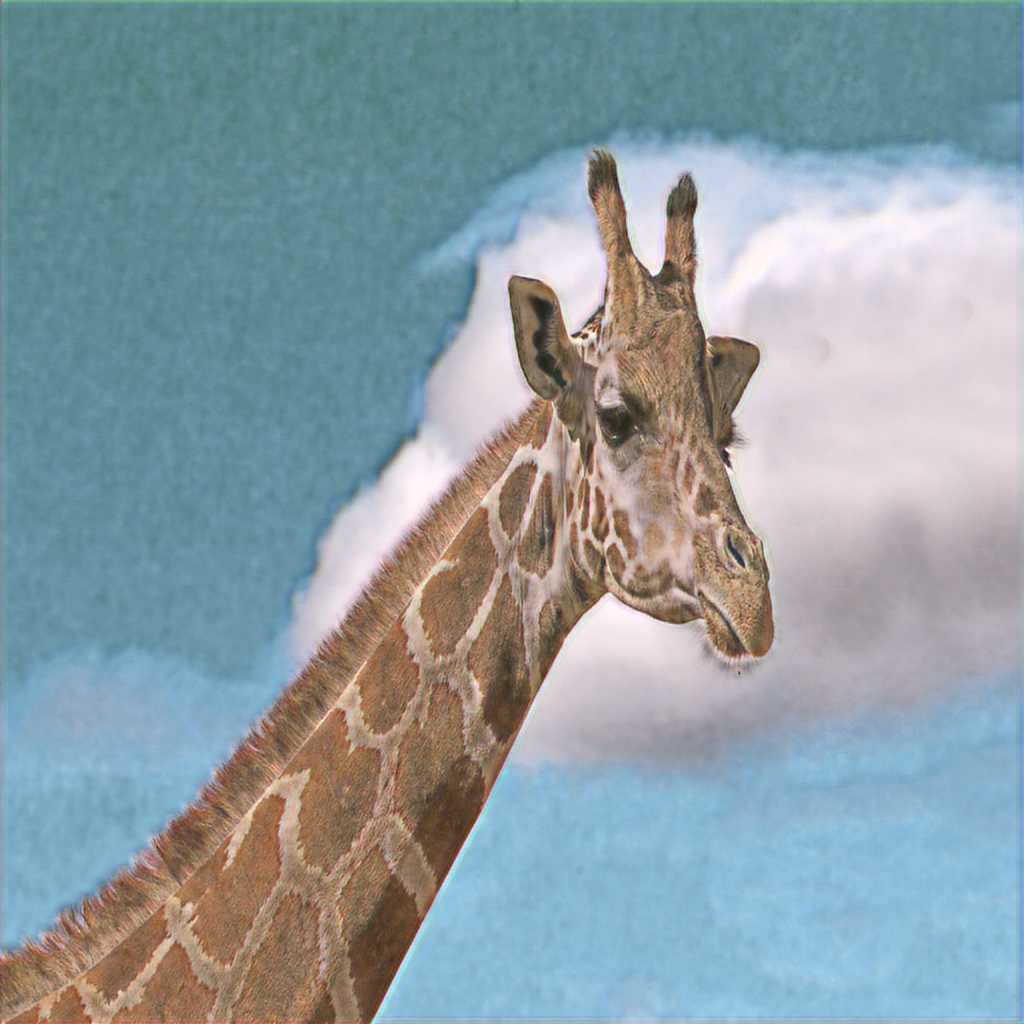
\includegraphics[width=\linewidth]{reconst_exper/dec_giraffe_my_2_test.png} % our reconstruction arc2 num.1	
	\end{subfigure}
	\begin{subfigure}[b]{0.13\linewidth}
		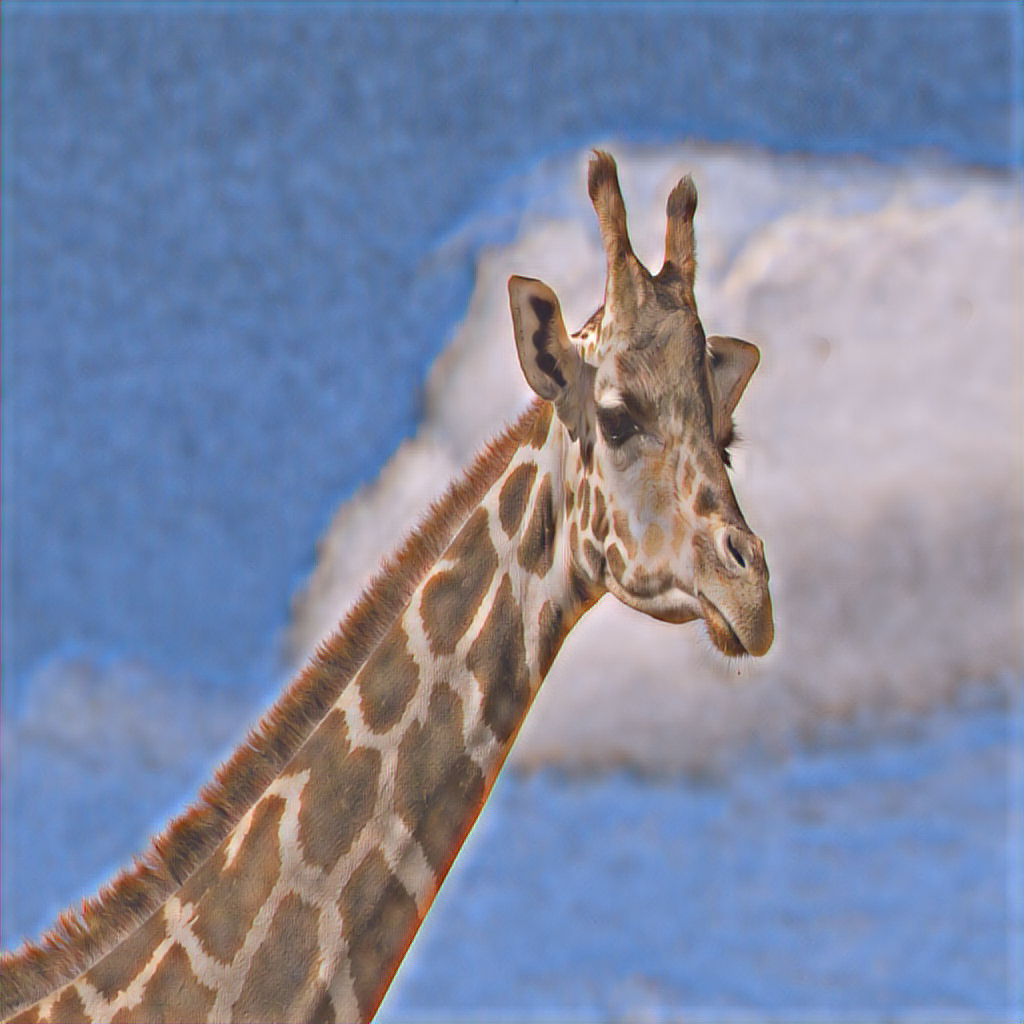
\includegraphics[width=\linewidth]{reconst_exper/dec_giraffe_my_3_test.png} % our reconstruction arc3 num.1	
	\end{subfigure}
	\begin{subfigure}[b]{0.13\linewidth}
		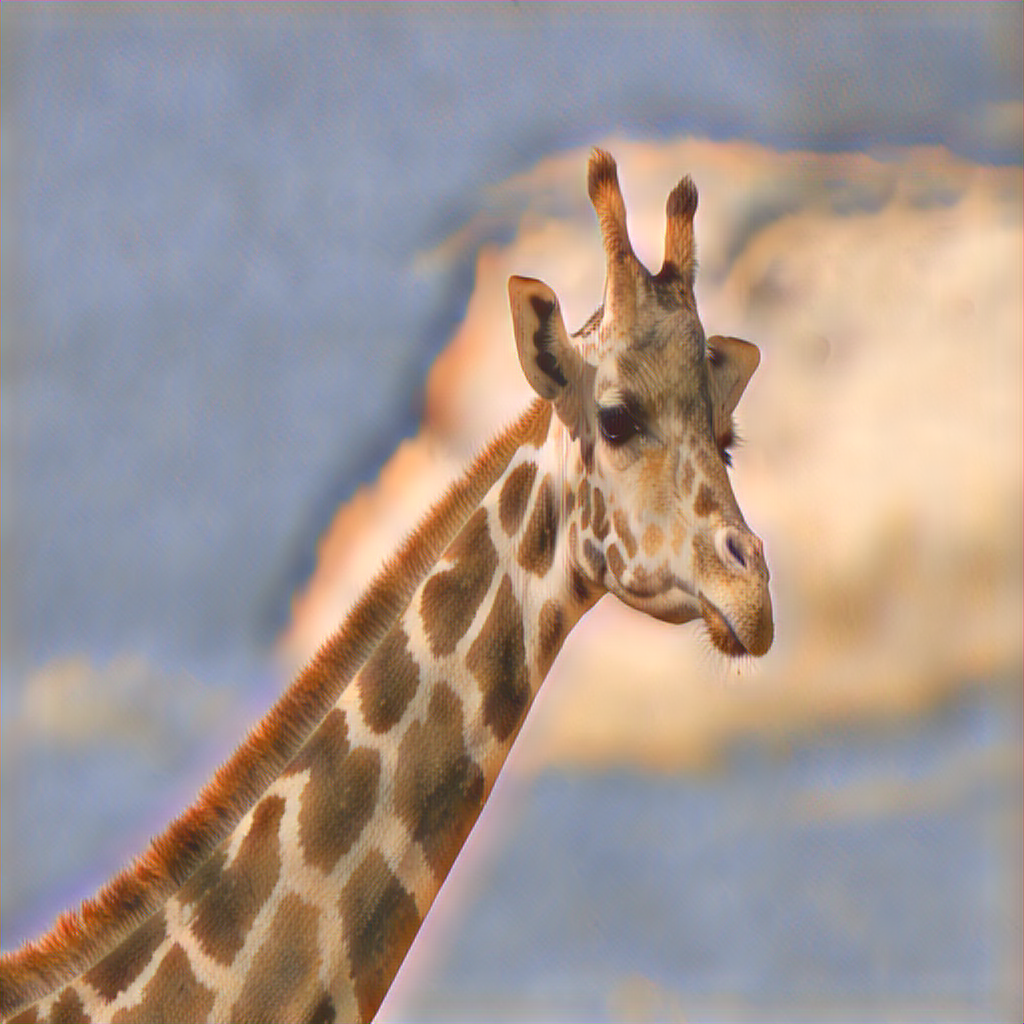
\includegraphics[width=\linewidth]{reconst_exper/dec_giraffe_my_4_test.png} % our reconstruction arc4 num.1	
	\end{subfigure}
	\begin{subfigure}[b]{0.13\linewidth}
		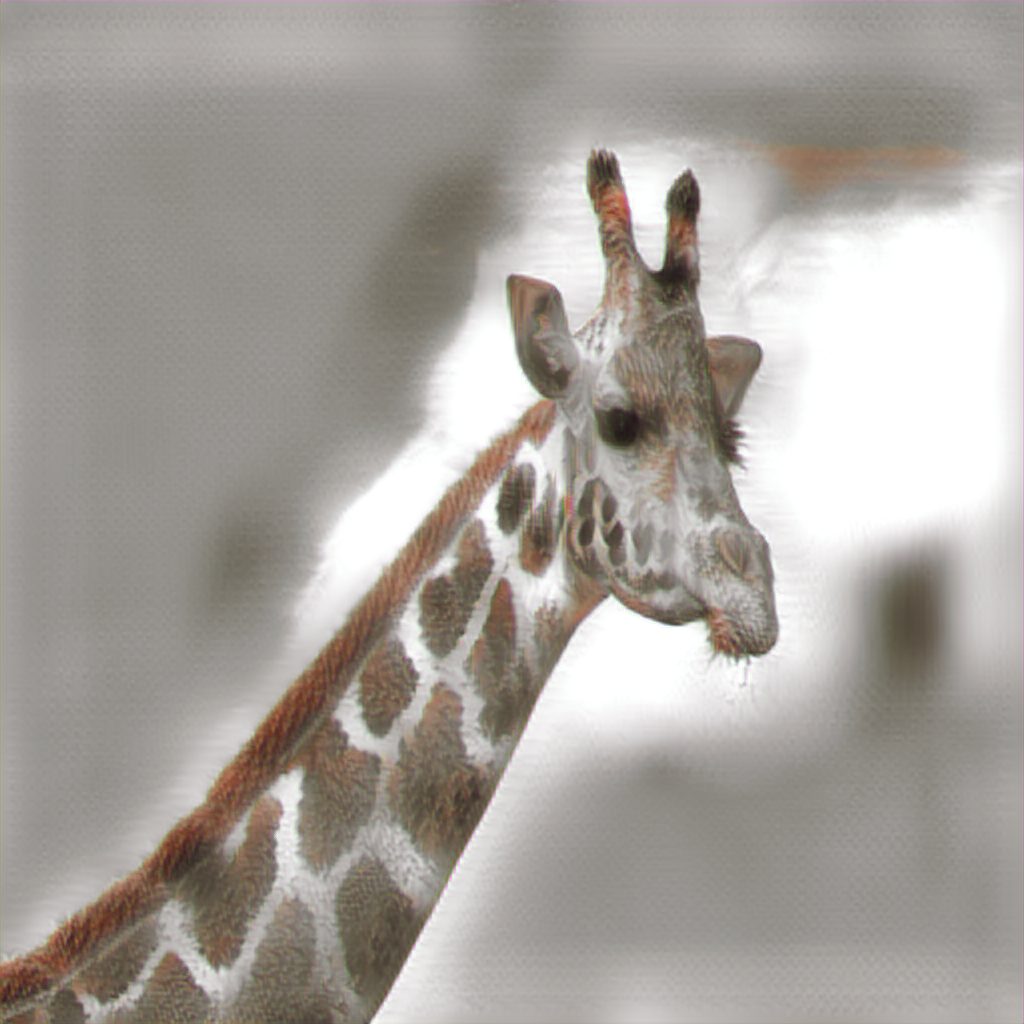
\includegraphics[width=\linewidth]{reconst_exper/dec_giraffe_my_5_test.png} % our reconstruction arc5 num.1	
	\end{subfigure}
	\begin{subfigure}[b]{0.13\linewidth}
		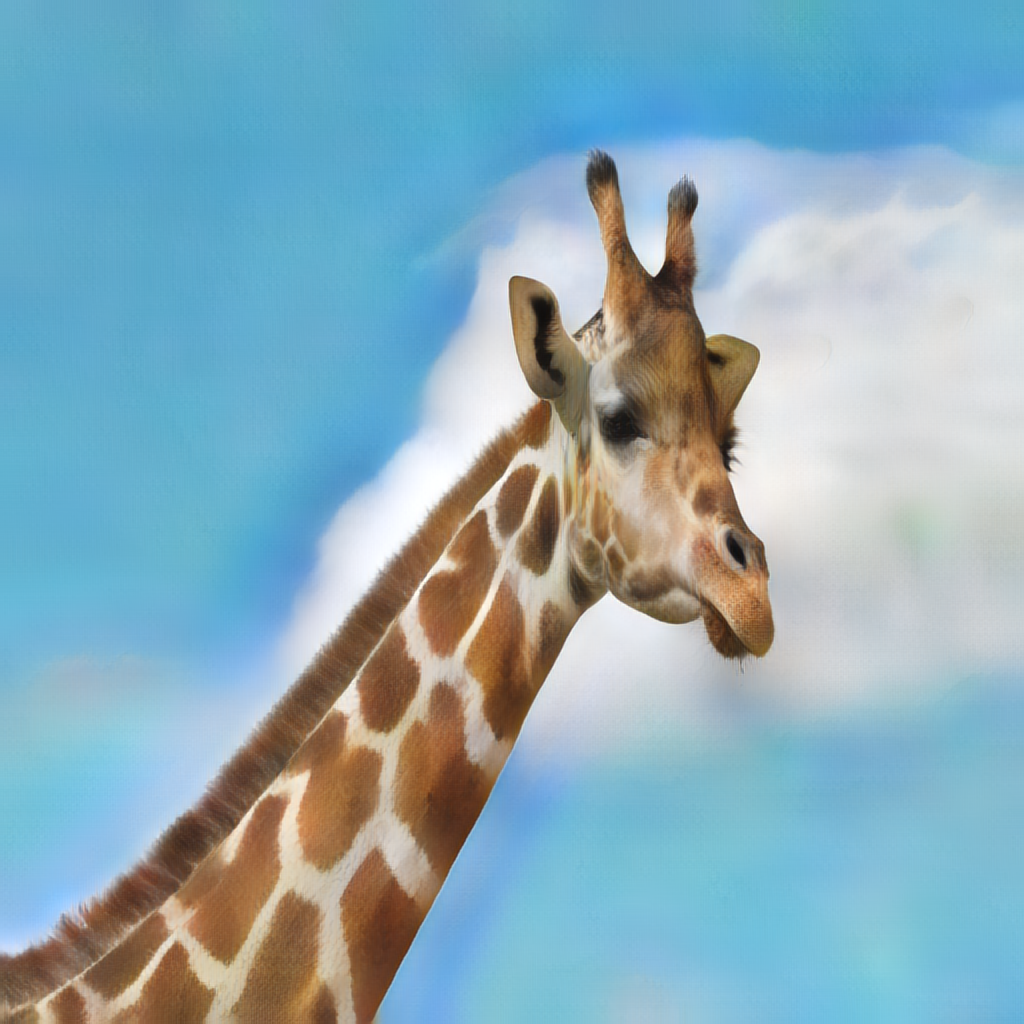
\includegraphics[width=\linewidth]{reconst_exper/dec_giraffe_ref_5_test.png} % their reconstruction arc5 num.1	
	\end{subfigure}
	% third line
	\centering
	\begin{subfigure}[b]{0.13\linewidth}
		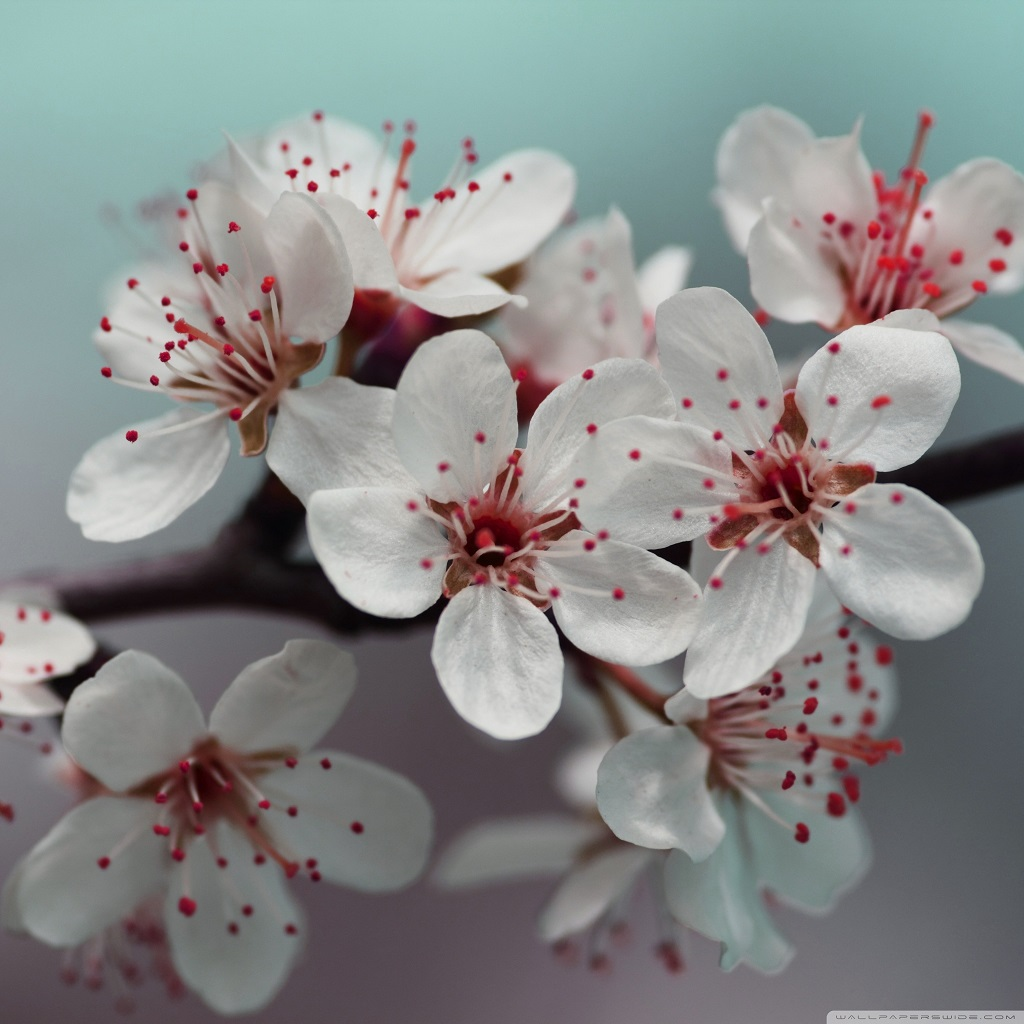
\includegraphics[width=\linewidth]{in1_sq.jpg} % original num.1	
	\end{subfigure}
	\begin{subfigure}[b]{0.13\linewidth}
		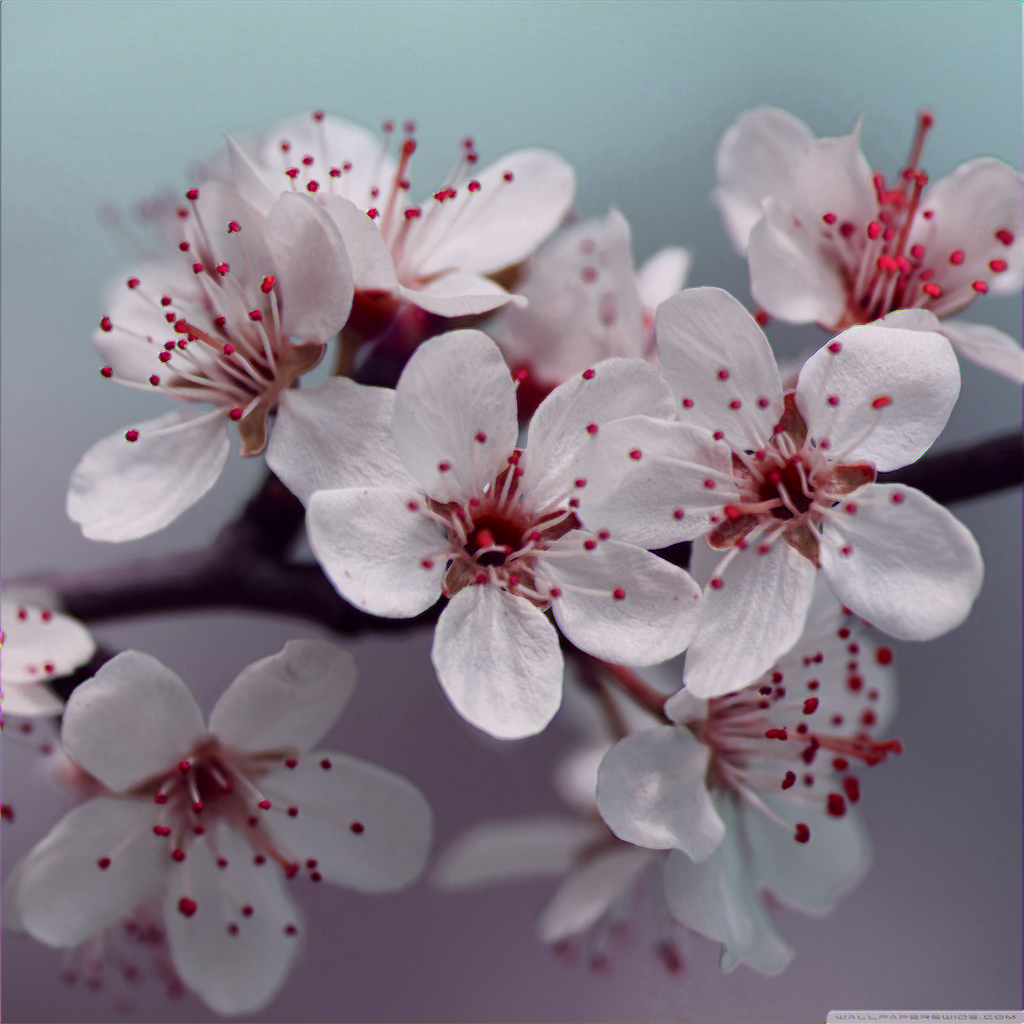
\includegraphics[width=\linewidth]{reconst_exper/dec_in1_my_1_test.png} % our reconstruction arc1 num.1	
	\end{subfigure}
	\begin{subfigure}[b]{0.13\linewidth}
		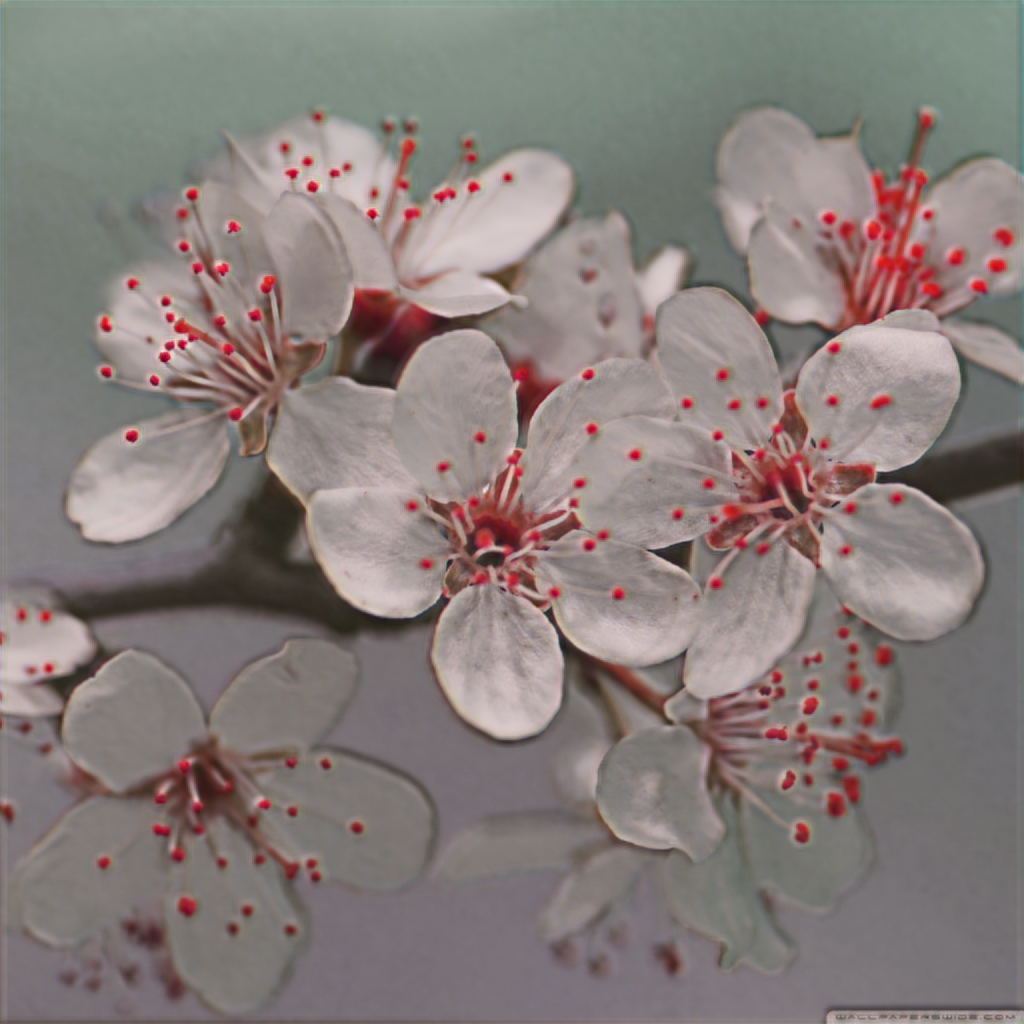
\includegraphics[width=\linewidth]{reconst_exper/dec_in1_my_2_test.png} % our reconstruction arc2 num.1	
	\end{subfigure}
	\begin{subfigure}[b]{0.13\linewidth}
		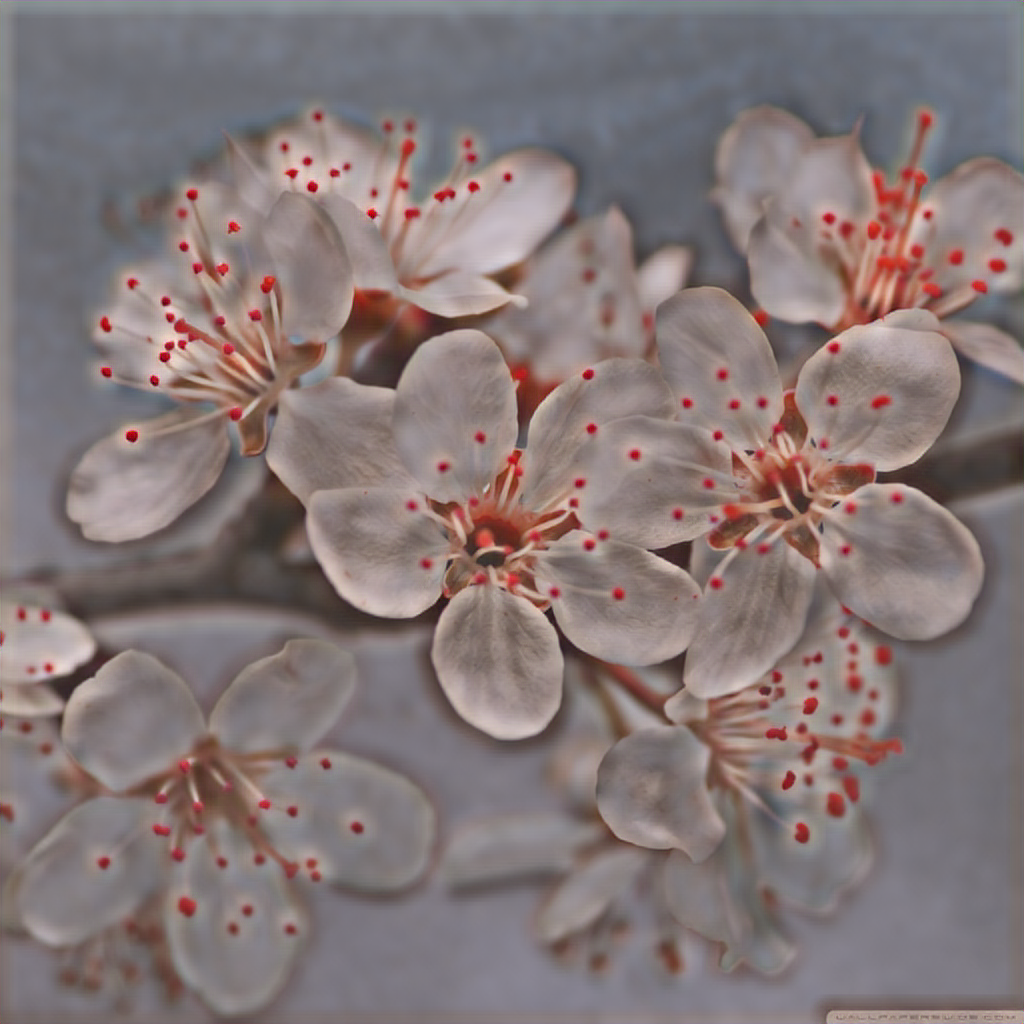
\includegraphics[width=\linewidth]{reconst_exper/dec_in1_my_3_test.png} % our reconstruction arc3 num.1	
	\end{subfigure}
	\begin{subfigure}[b]{0.13\linewidth}
		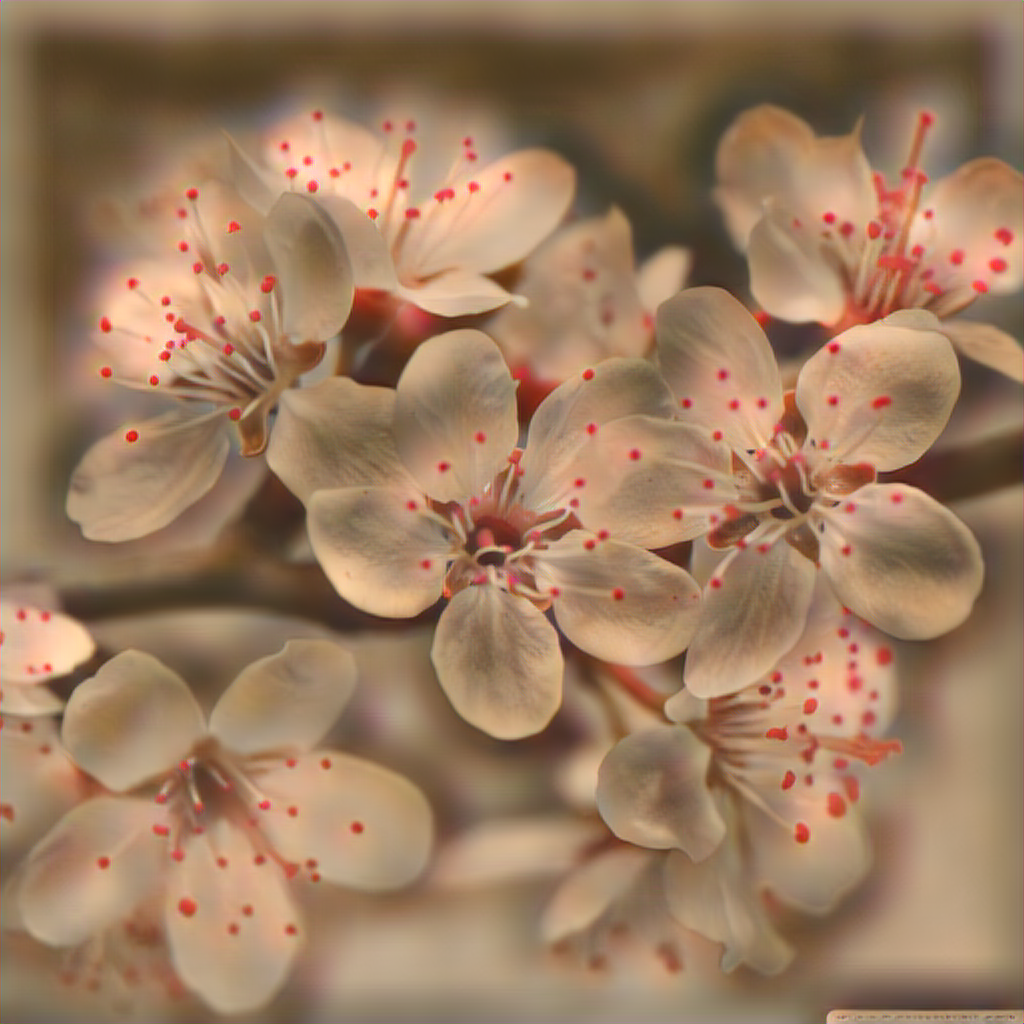
\includegraphics[width=\linewidth]{reconst_exper/dec_in1_my_4_test.png} % our reconstruction arc4 num.1	
	\end{subfigure}
	\begin{subfigure}[b]{0.13\linewidth}
		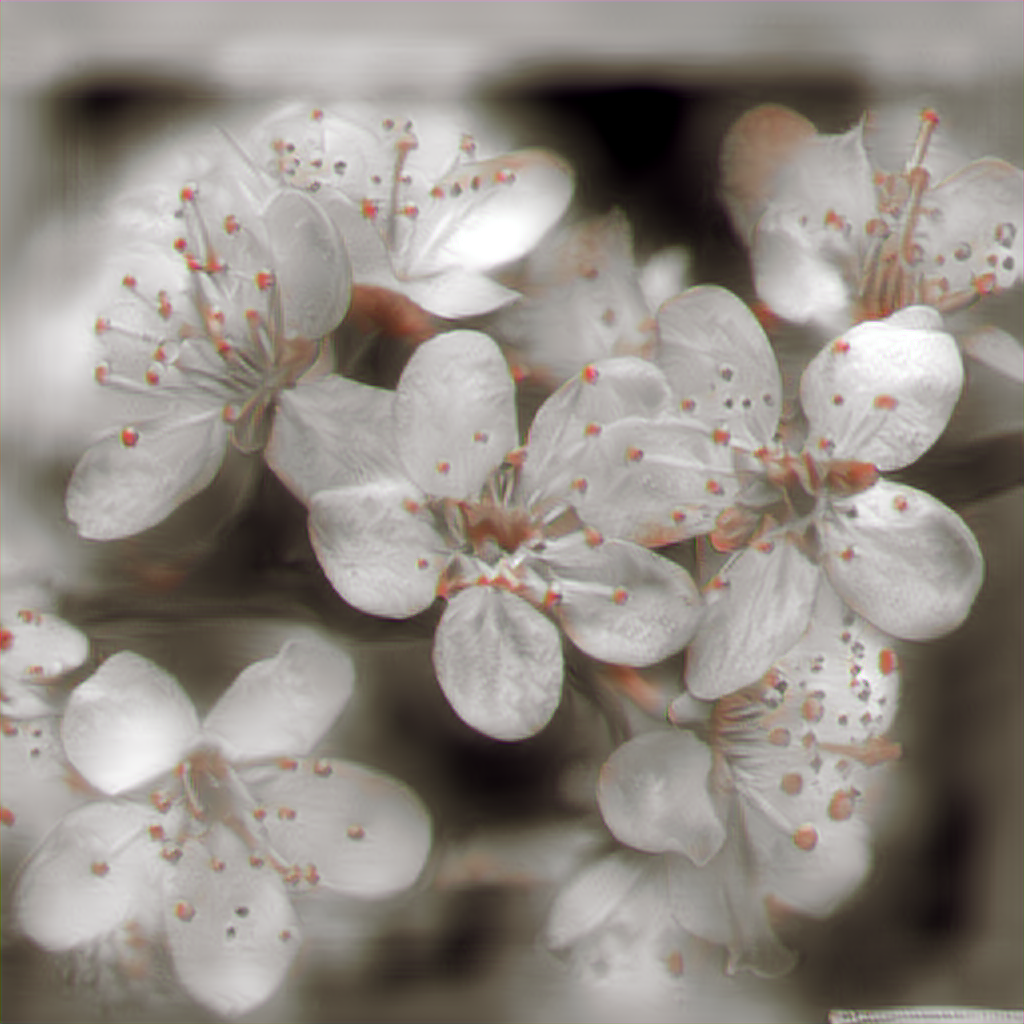
\includegraphics[width=\linewidth]{reconst_exper/dec_in1_my_5_test.png} % our reconstruction arc5 num.1	
	\end{subfigure}
	\begin{subfigure}[b]{0.13\linewidth}
		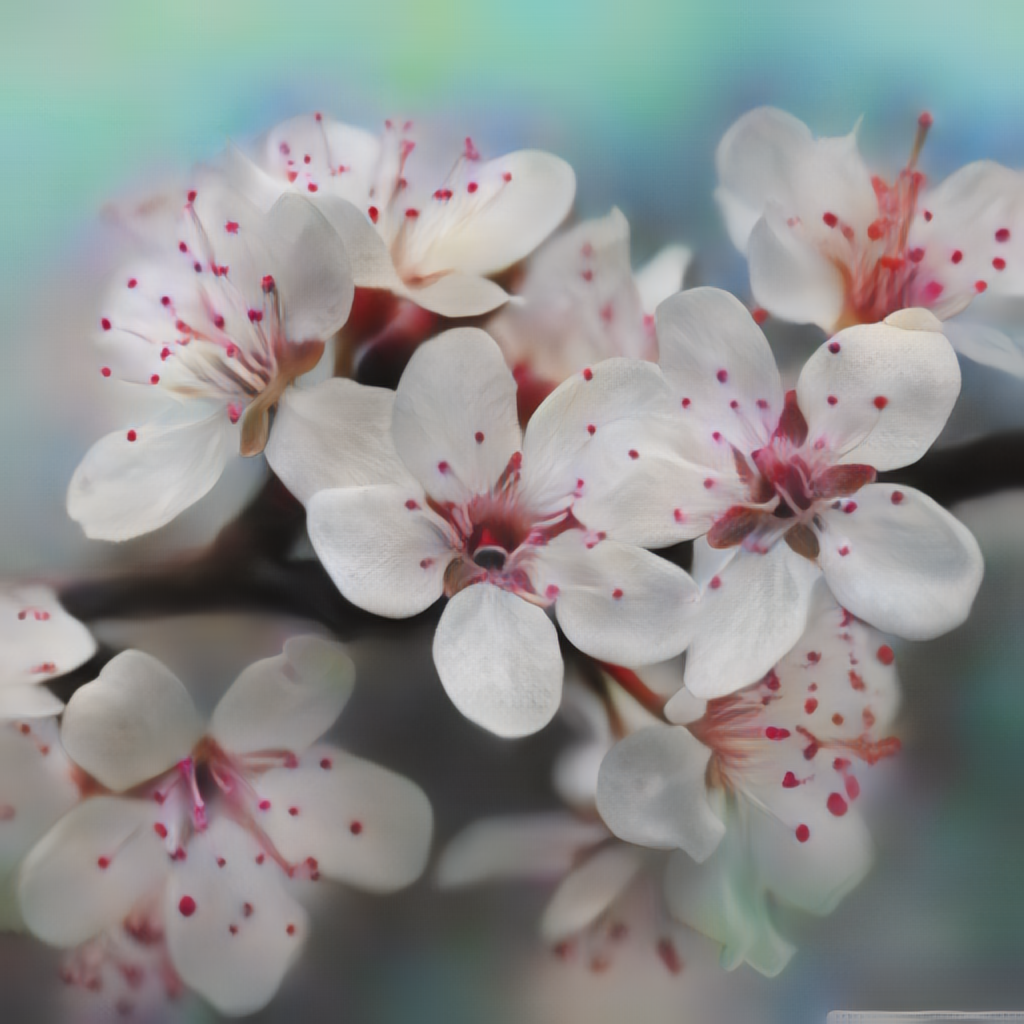
\includegraphics[width=\linewidth]{reconst_exper/dec_in1_ref_5_test.png} % their reconstruction arc5 num.1	
	\end{subfigure}
	%fourth line
	\centering
	\begin{subfigure}[b]{0.13\linewidth}
		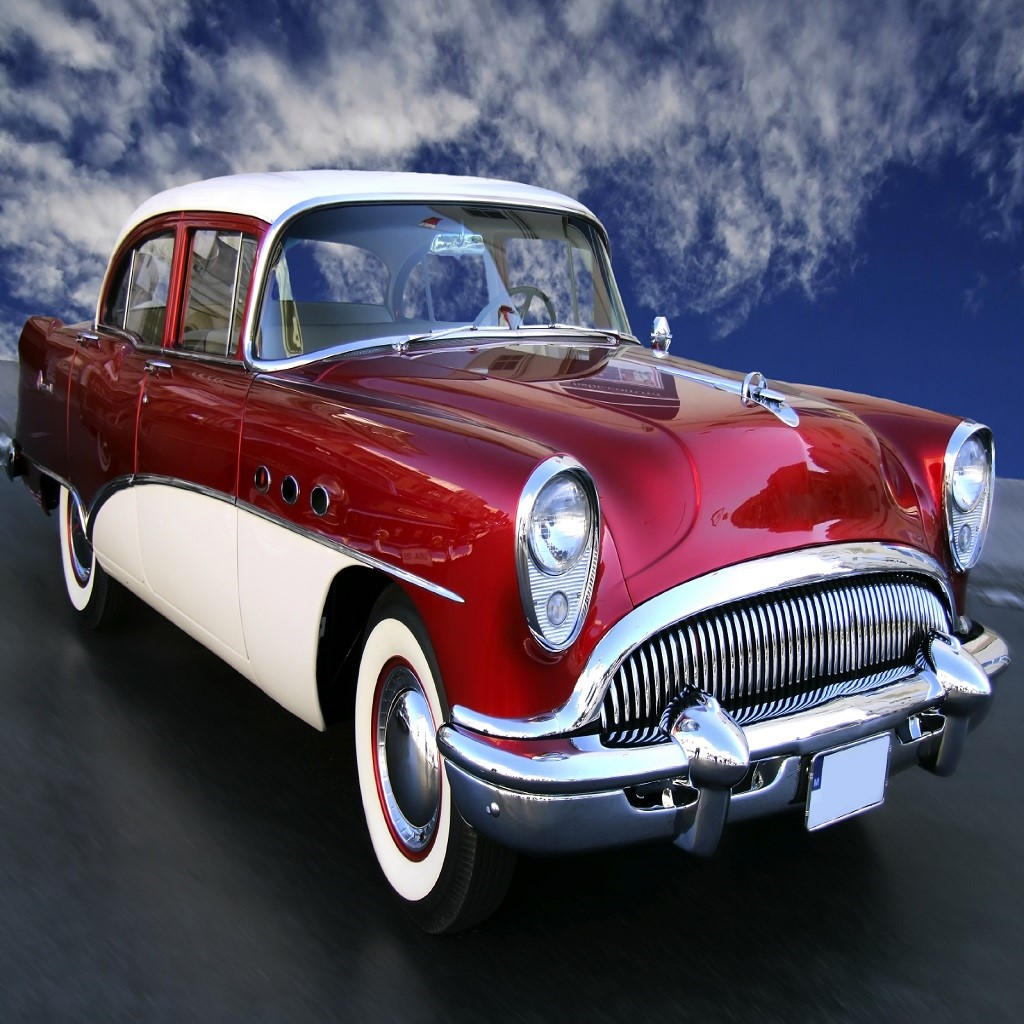
\includegraphics[width=\linewidth]{car_sq.jpg} % original num.1	
	\end{subfigure}
	\begin{subfigure}[b]{0.13\linewidth}
		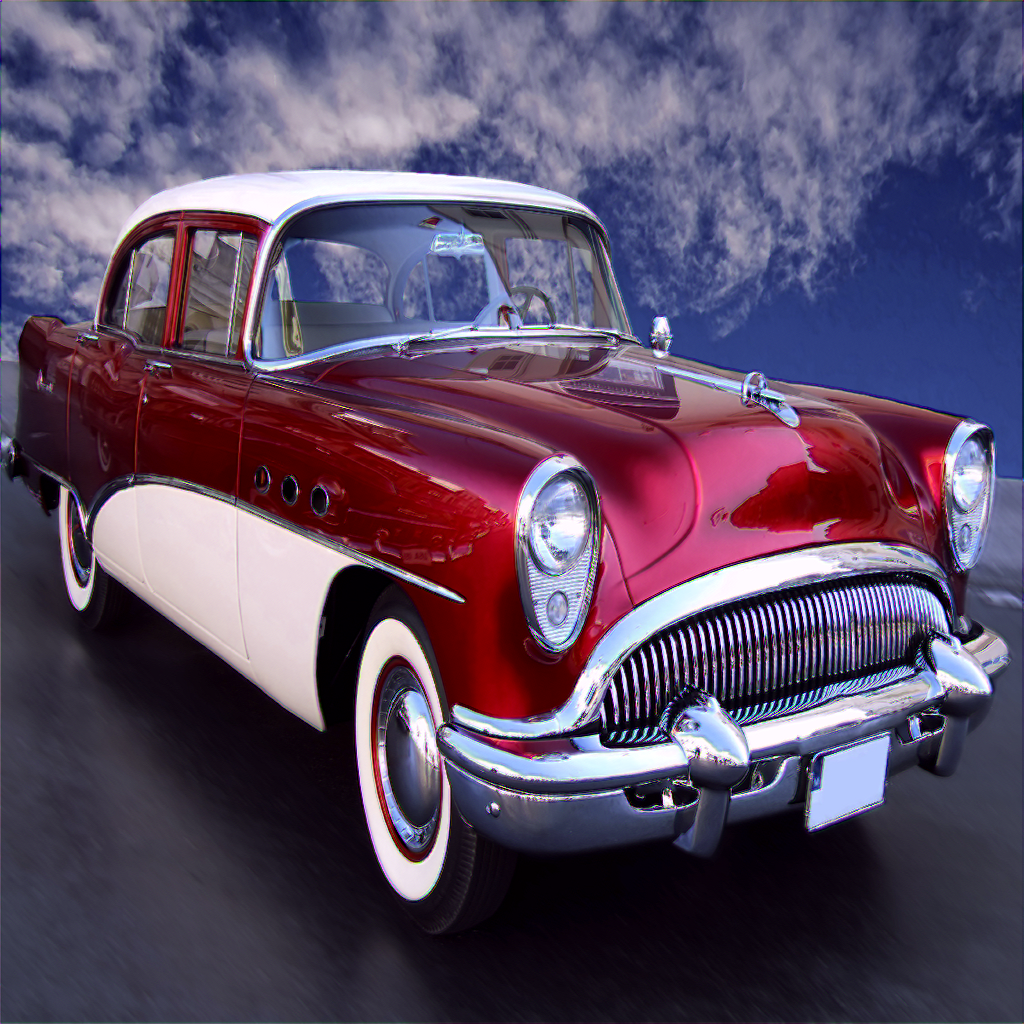
\includegraphics[width=\linewidth]{reconst_exper/dec_in2_my_1_test.png} % our reconstruction arc1 num.1	
	\end{subfigure}
	\begin{subfigure}[b]{0.13\linewidth}
		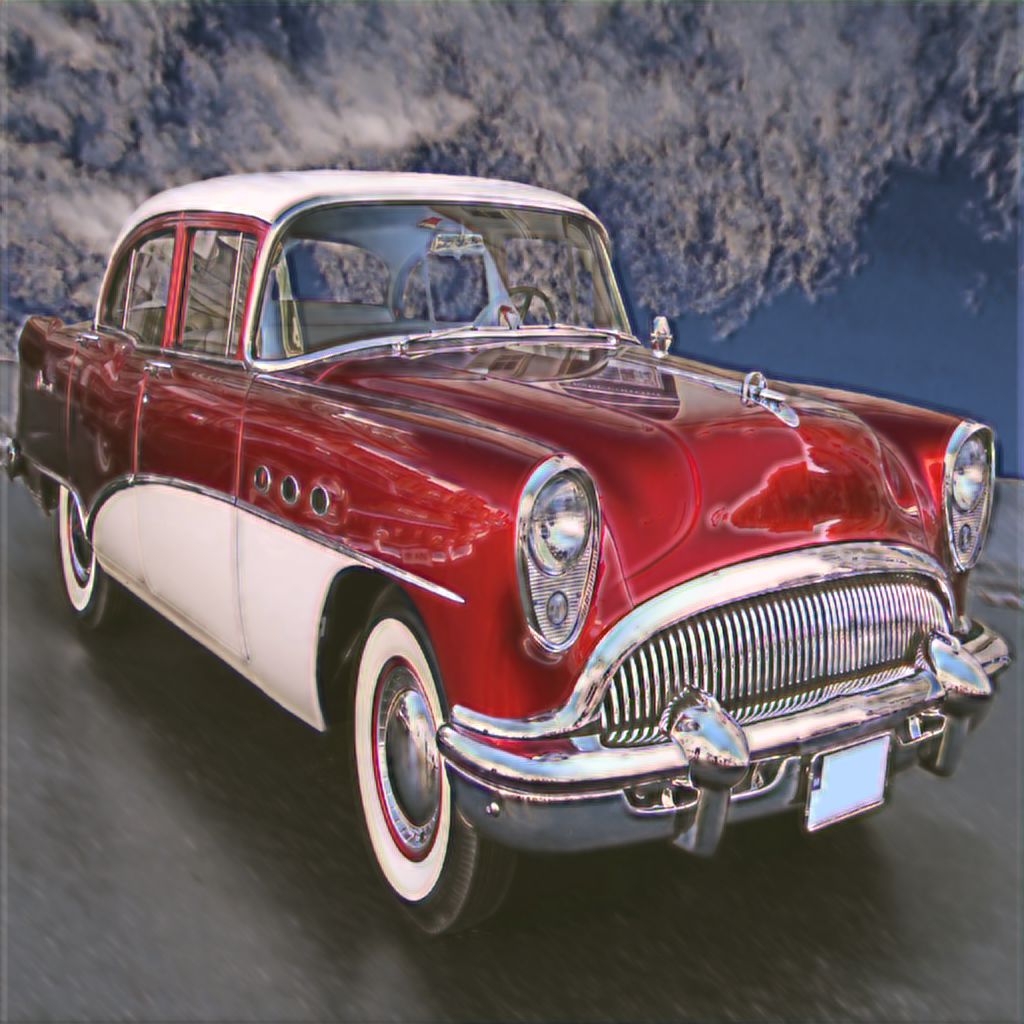
\includegraphics[width=\linewidth]{reconst_exper/dec_in2_my_2_test.png} % our reconstruction arc2 num.1	
	\end{subfigure}
	\begin{subfigure}[b]{0.13\linewidth}
		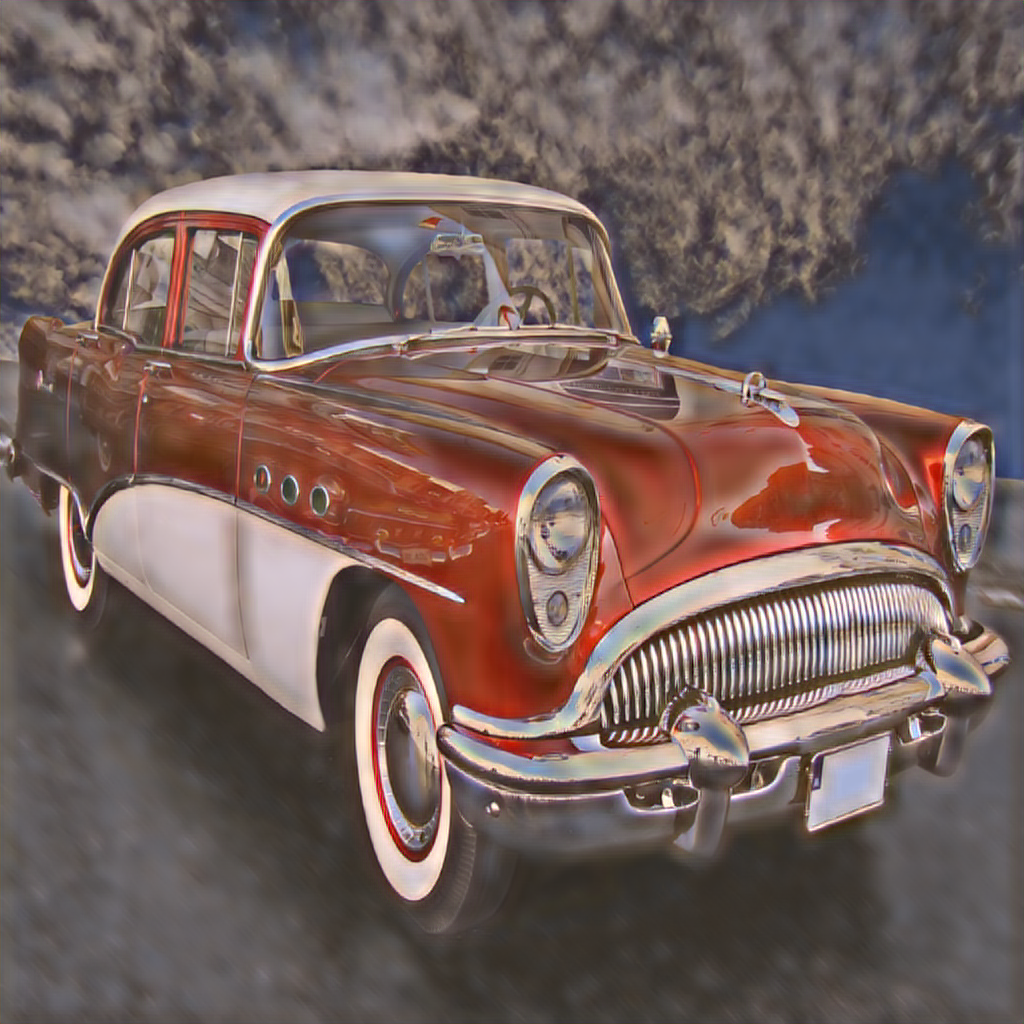
\includegraphics[width=\linewidth]{reconst_exper/dec_in2_my_3_test.png} % our reconstruction arc3 num.1	
	\end{subfigure}
	\begin{subfigure}[b]{0.13\linewidth}
		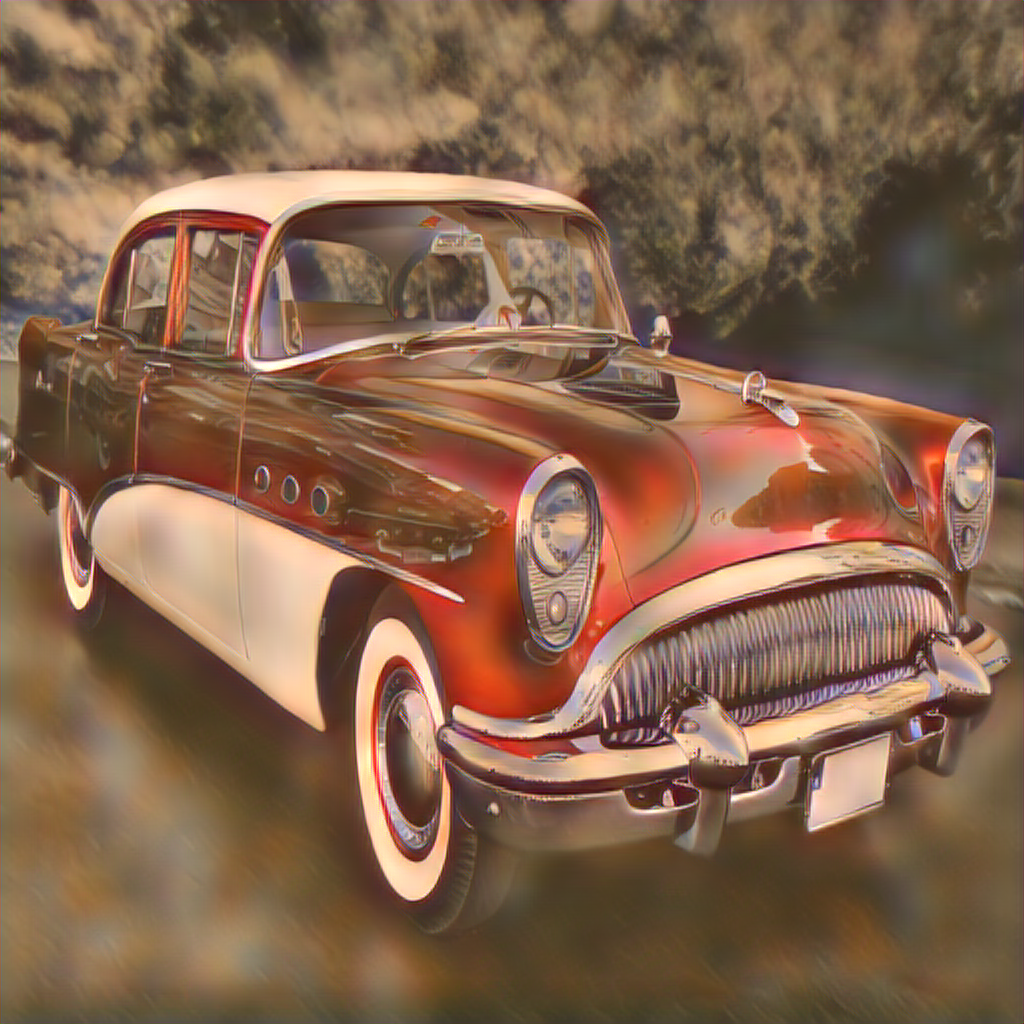
\includegraphics[width=\linewidth]{reconst_exper/dec_in2_my_4_test.png} % our reconstruction arc4 num.1	
	\end{subfigure}
	\begin{subfigure}[b]{0.13\linewidth}
		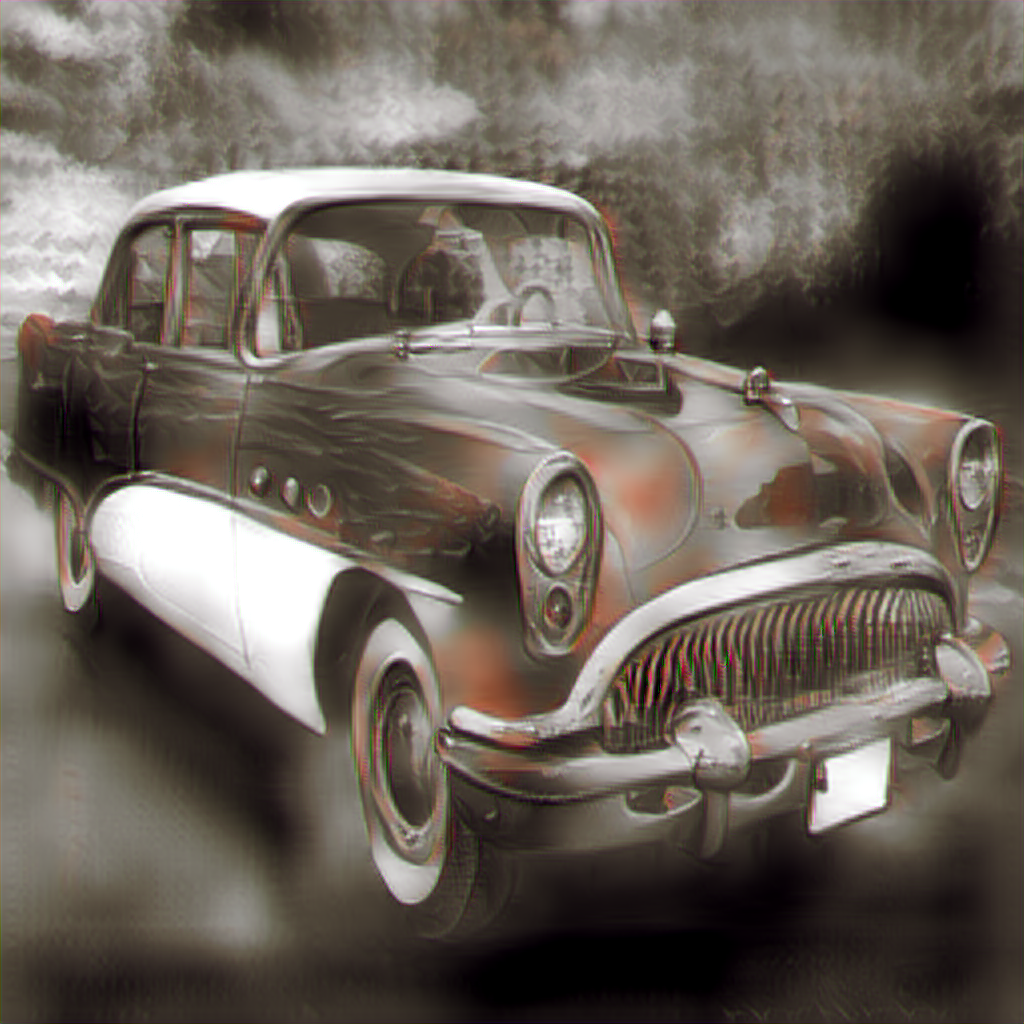
\includegraphics[width=\linewidth]{reconst_exper/dec_in2_my_5_test.png} % our reconstruction arc5 num.1	
	\end{subfigure}
	\begin{subfigure}[b]{0.13\linewidth}
		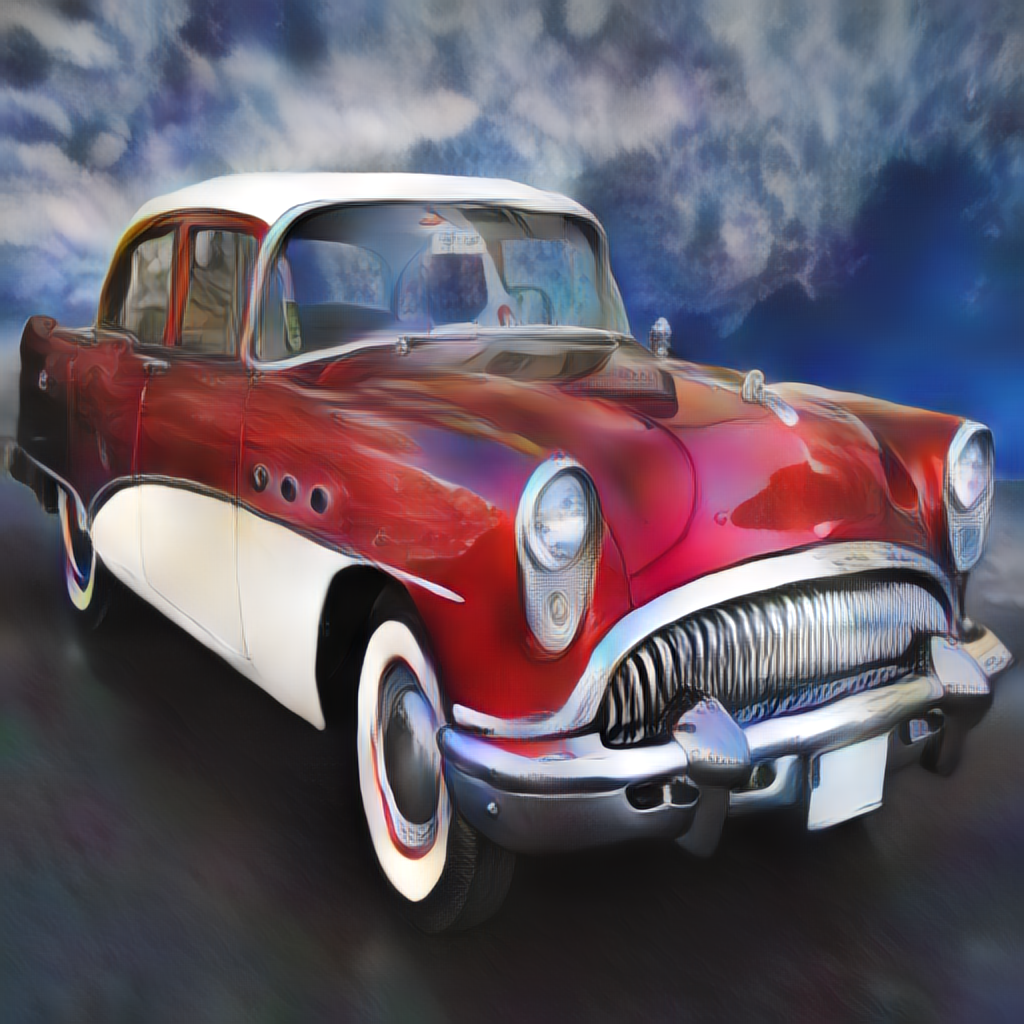
\includegraphics[width=\linewidth]{reconst_exper/dec_in2_ref_5_test.png} % their reconstruction arc5 num.1	
	\end{subfigure}
	% fifth line
	\centering
	\begin{subfigure}[b]{0.13\linewidth}
		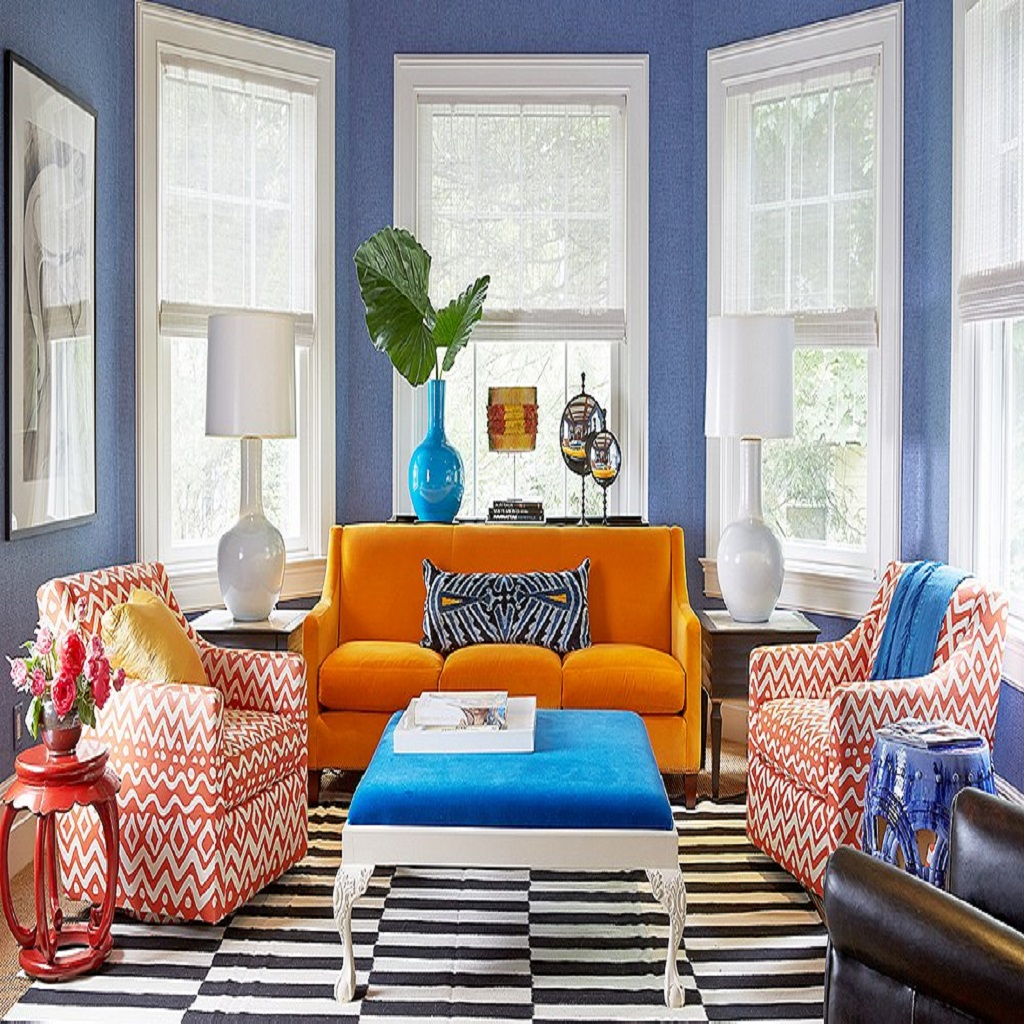
\includegraphics[width=\linewidth]{room_sq.jpg} % original num.5
		\caption{Original}
	\end{subfigure}
	\begin{subfigure}[b]{0.13\linewidth}
		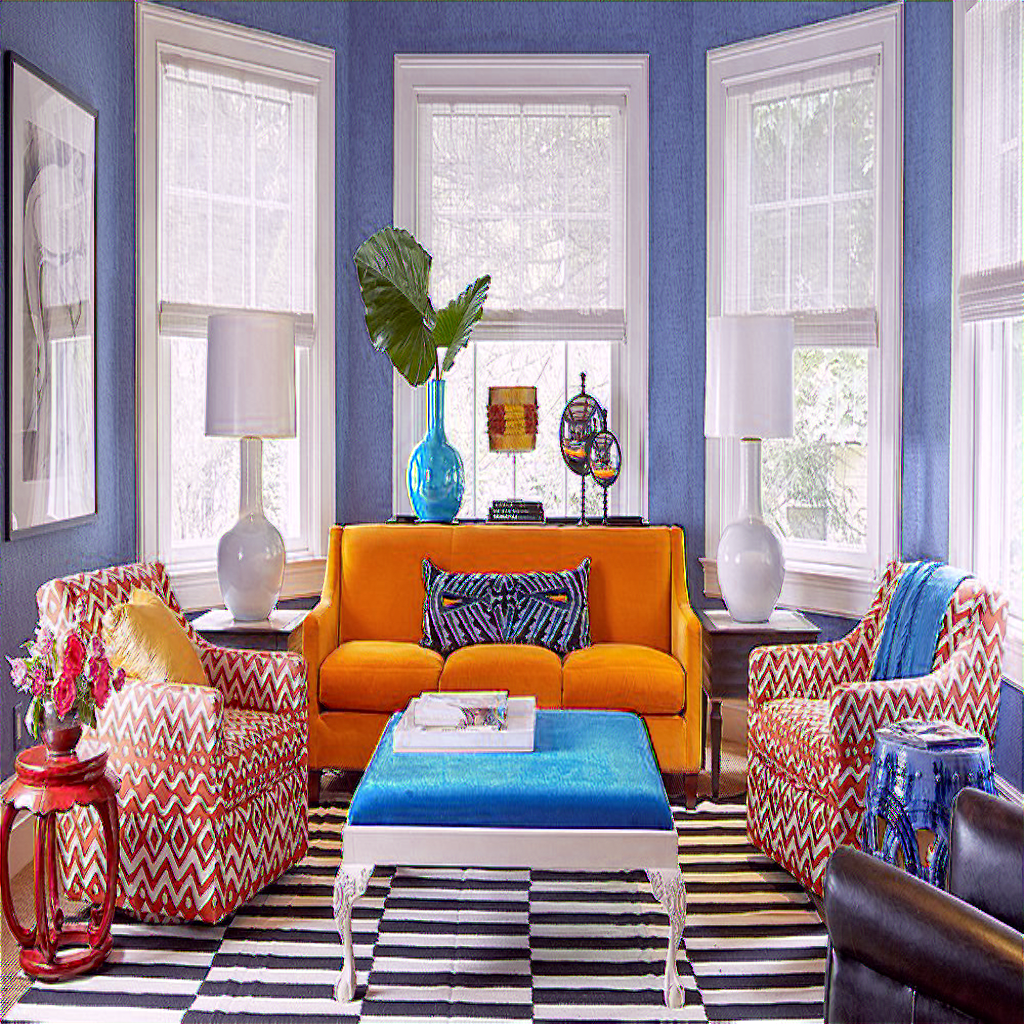
\includegraphics[width=\linewidth]{reconst_exper/dec_room_my_1_test.png} % our reconstruction num.5
		\caption{Ours arc1}
	\end{subfigure}
	\begin{subfigure}[b]{0.13\linewidth}
		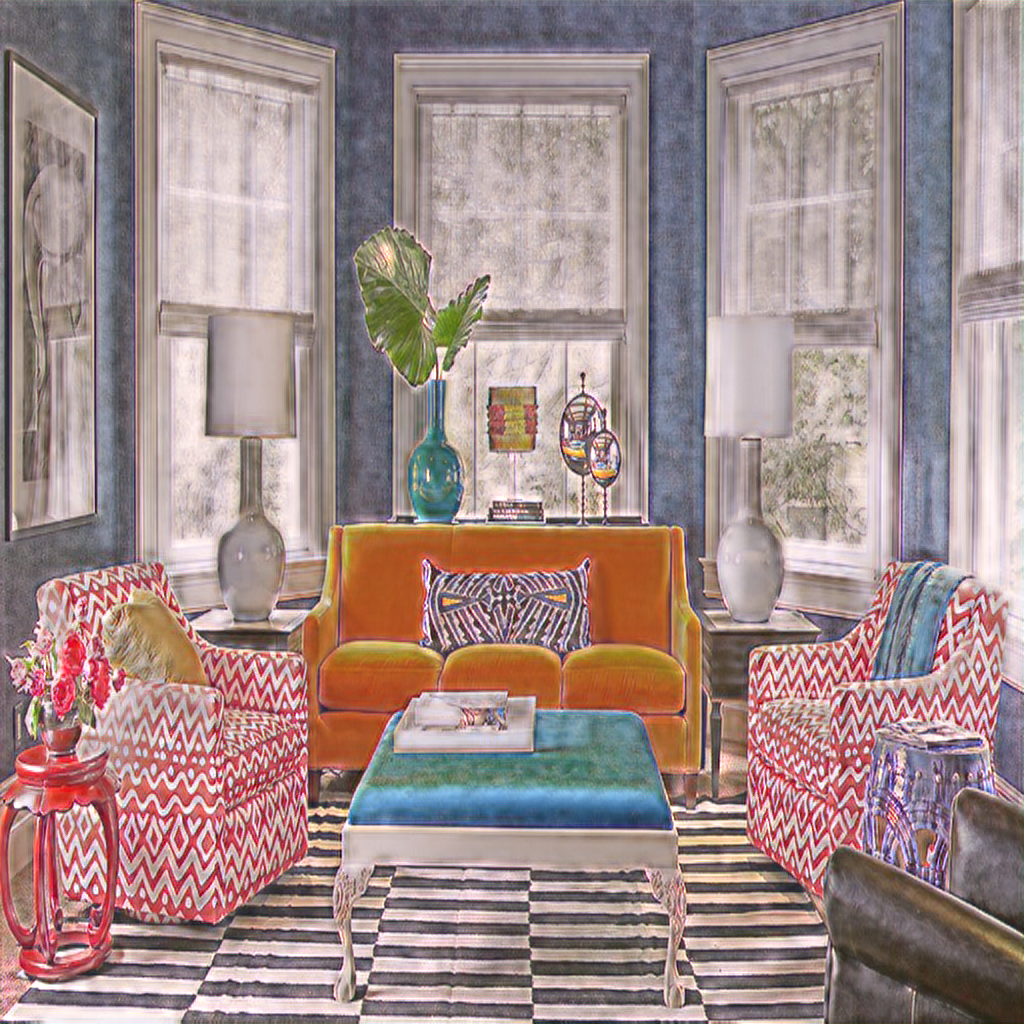
\includegraphics[width=\linewidth]{reconst_exper/dec_room_my_2_test.png} % our reconstruction num.5
		\caption{Ours arc2}
	\end{subfigure}
	\begin{subfigure}[b]{0.13\linewidth}
		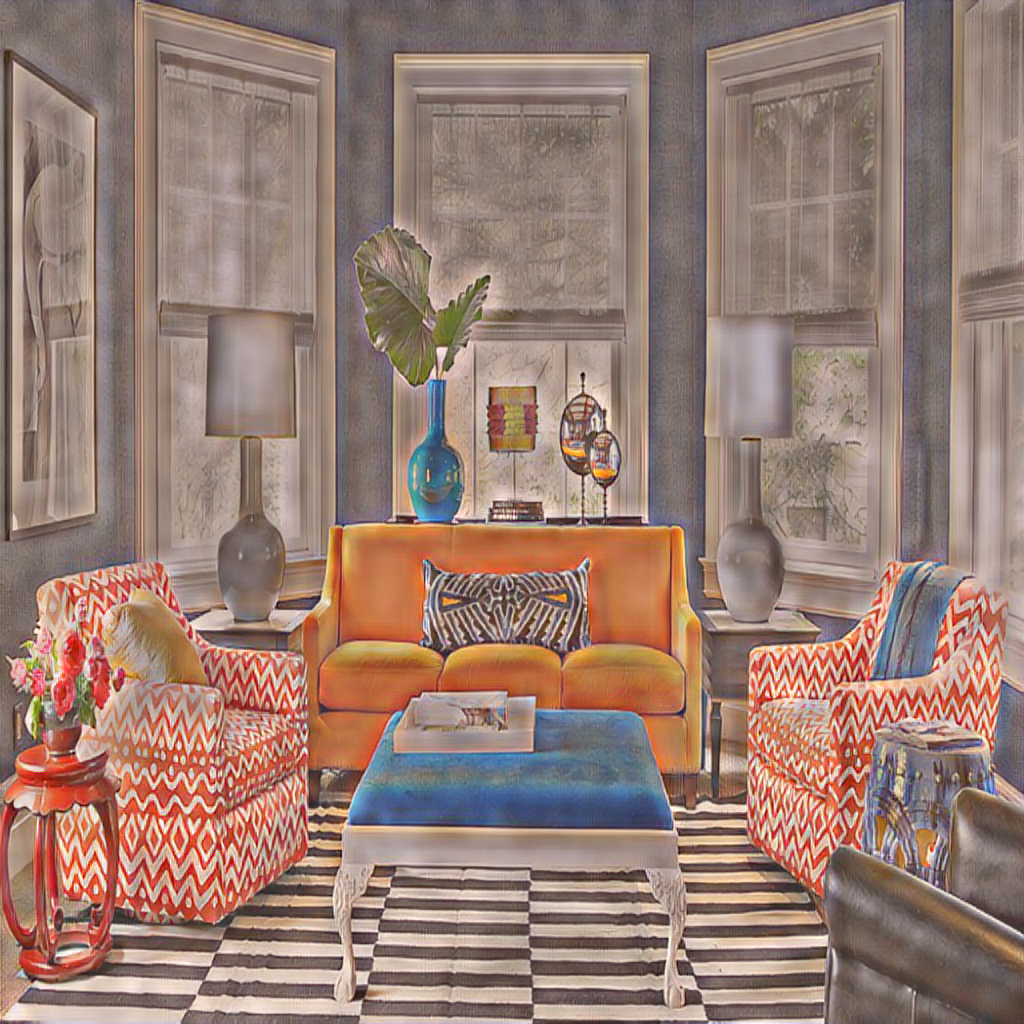
\includegraphics[width=\linewidth]{reconst_exper/dec_room_my_3_test.png} % our reconstruction num.5
		\caption{Ours arc3}
	\end{subfigure}
	\begin{subfigure}[b]{0.13\linewidth}
		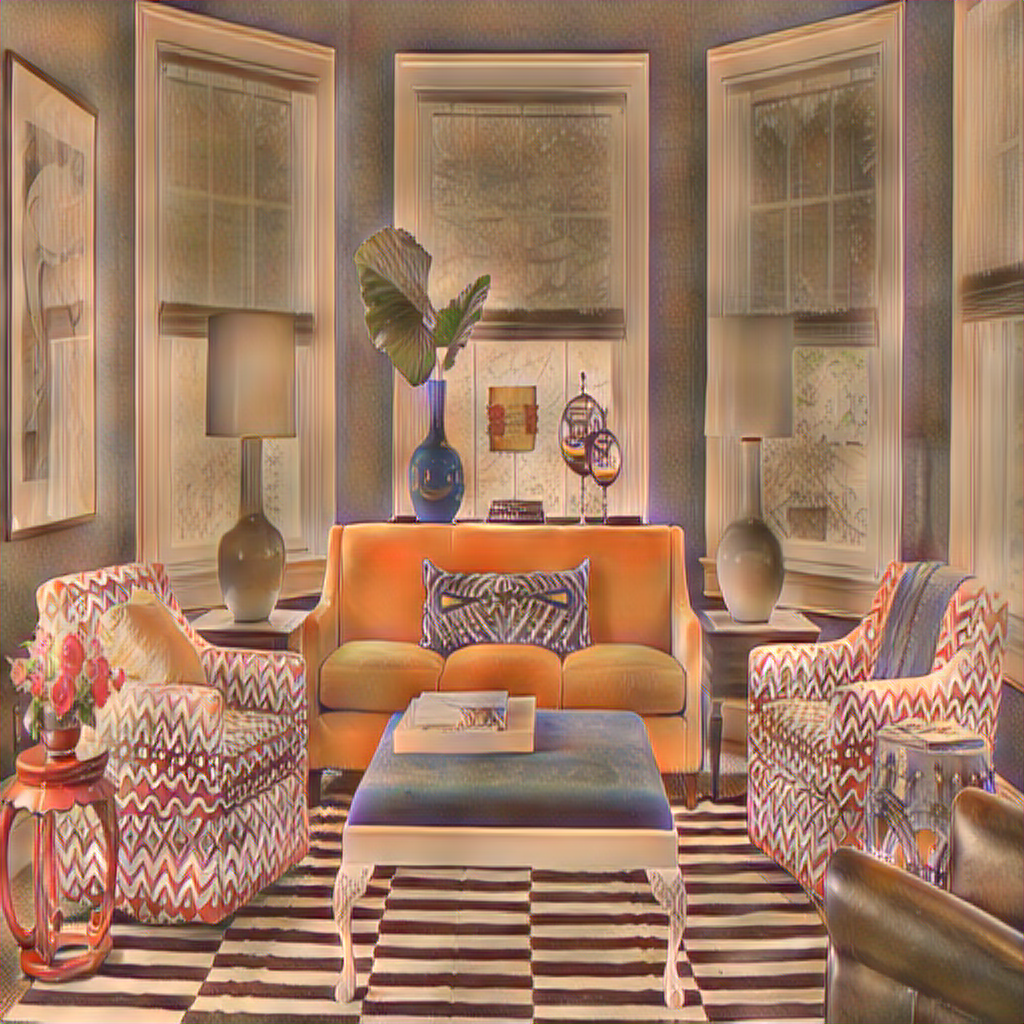
\includegraphics[width=\linewidth]{reconst_exper/dec_room_my_4_test.png} % our reconstruction num.5
		\caption{Ours arc4}
	\end{subfigure}
	\begin{subfigure}[b]{0.13\linewidth}
		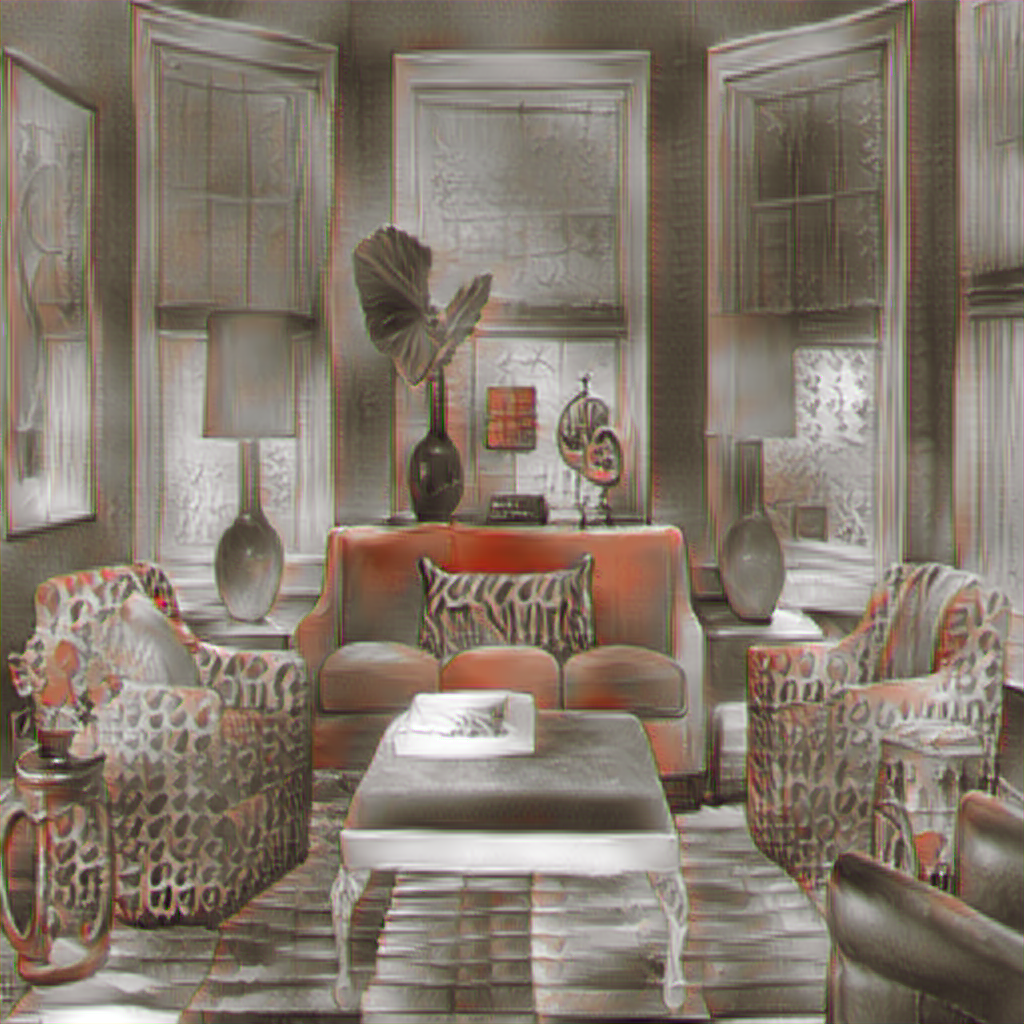
\includegraphics[width=\linewidth]{reconst_exper/dec_room_my_5_test.png} % our reconstruction num.5
		\caption{Ours arc5}
	\end{subfigure}
	\begin{subfigure}[b]{0.13\linewidth}
		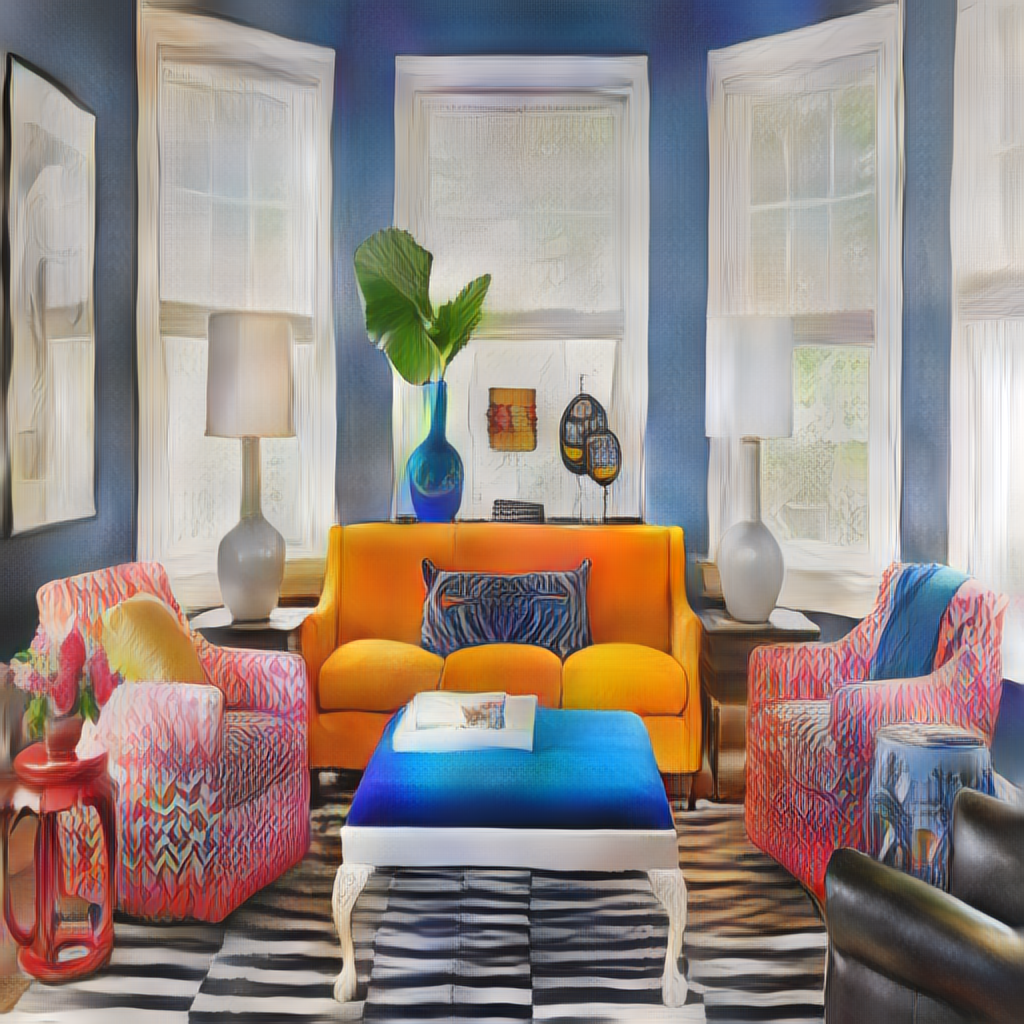
\includegraphics[width=\linewidth]{reconst_exper/dec_room_ref_5_test.png} % their reconstruction arc5 num.1
		\caption{Ref arc5}	
	\end{subfigure}
	\caption{Reconstructed images}
	\label{fig:reconstruction}
\end{figure}
Figure ~\ref{fig:reconstruction} shows reconstruction of original images (figure ~\ref{fig:reconstruction} (a)) using different architectures of encoder-decoder, i.e. figure ~\ref{fig:reconstruction} (b) uses architecture 1 which uses Encoder-1 and Decoder-Block-1, figure ~\ref{fig:reconstruction} (c) uses architecture 3 which uses Encoder-3 and Decoder-Block-3, etc. as depicted in \ref{subsec:Models}.

\subsubsection{TODO}
Our distortion-of-reconstruction loss table ~\ref{Tab:loss} shows by both pixel and feature loss, that the first architecture has the less loss since it is only uses 1 convolution layer. As we go deeper in architectures in a manner of convolutional layers, we see that the loss arises respectively. Hence we decided to balance the distortion in out continuous work, therefore we chose to work with a pipeline that has architecture 4, forsake architecture 5 to avoid major distortion such as smoothing and blurring artifacts.

As part of implementing UST \cite{bib11}, we separately train five reconstruction decoders for features
at the VGG-19 \verb|Relu_X_1| (X=1,2,...,5) layers. It is trained on the Microsoft COCO dataset \cite{bib10} and
the weight $\lambda$ to balance the two losses in (2) is set as 1.
The pixel reconstruction loss \cite{bib22} and feature loss \cite{bib22, bib17} are employed for reconstructing an input image, see equation ~\ref{eq:loss}
After training, the decoder is fixed (i.e., will not be fine-tuned) and used as a feature inverter.\newline
%%%%%%%%%%%%%%%%%%%%%%%%%%%%%%%%%%%%%%%%%%
%%% recunstruction comparison %%%
%%%%%%%%%%%%%%%%%%%%%%%%%%%%%%%%%%%%%%%%%%
Section \ref{subsec:Decoders} explains why we needed to train 5 different decoders. Without time and compute power limitations we could get much more powerful decoders which are not producing such as artifacts.
In addition, we measure quantitatively (see table ~\ref{Tab:loss}) our reconstruction distortion loss by two measures: pixel loss and feature loss as depicted in equation \ref{eq:loss} and elaborated in \cite{bib22, bib17}.\newline\\

%%%%%%%%%%%%%%%%%%%%%%%%%%%%%% Reconstrucion images %%%%%%%%%%%%%%%%%%%%%%%%%%%%%%%%%%

  
%%%%%%%%%%%%%%%%%%%%%%%%%%%%
%%%%%%%%%%%%%%%%%%%%%%%%%%%%
% style transfer images %
%%%%%%%%%%%%%%%%%%%%%%%%%%%%
%%%%%%%%%%%%%%%%%%%%%%%%%%%%
\subsection{Style Transfer Experimental Results}
\begin{figure}[H]
	% first line
	\centering
	\begin{subfigure}[b]{0.225\linewidth}
		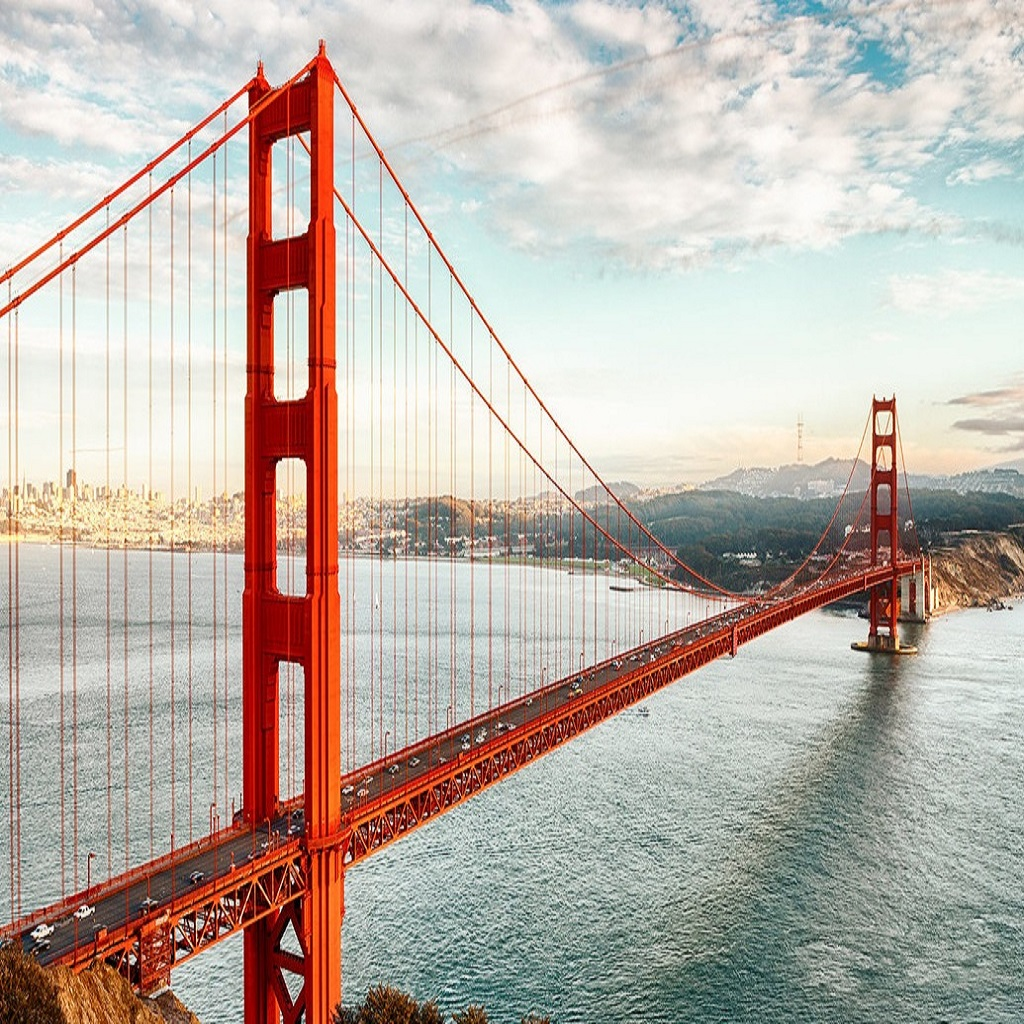
\includegraphics[width=\linewidth]{bridge_sq.jpg} % style img num.1
	\end{subfigure}
	\begin{subfigure}[b]{0.225\linewidth}
		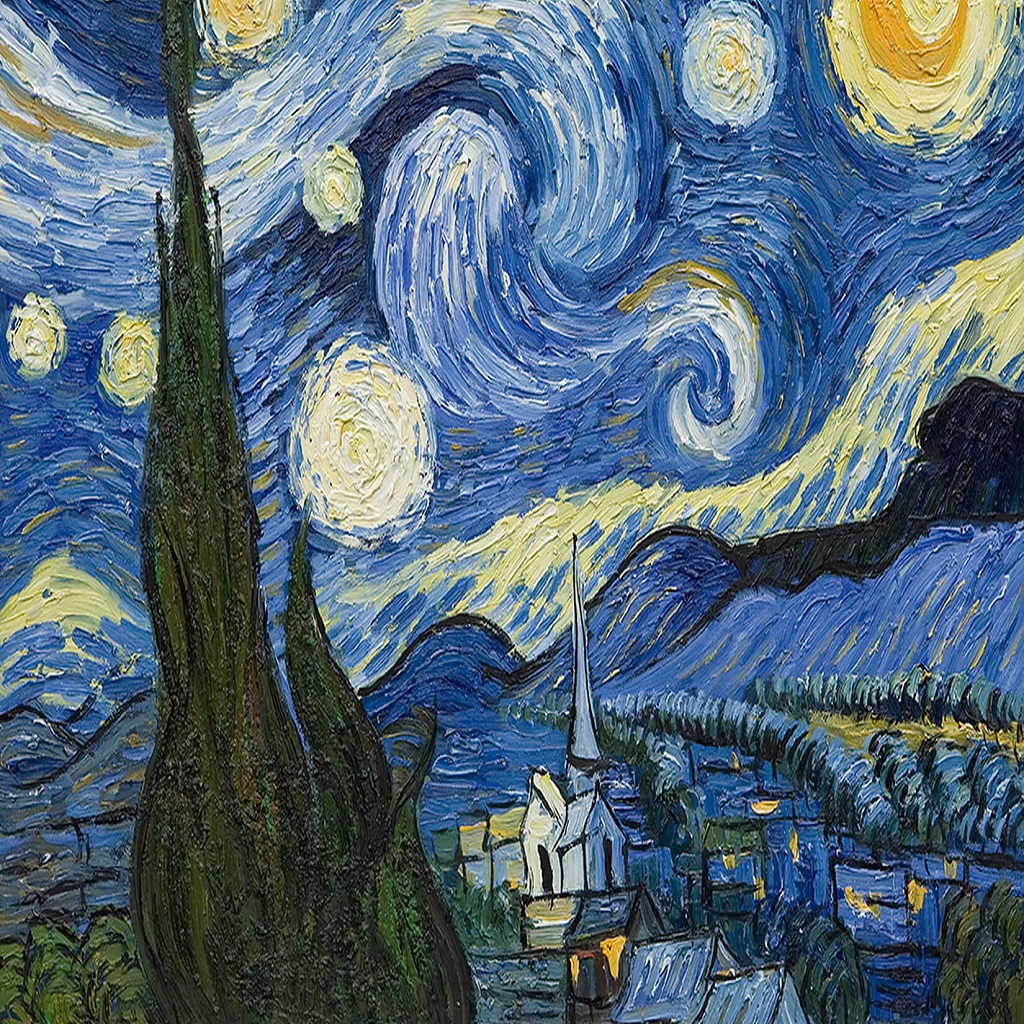
\includegraphics[width=\linewidth]{starry_sq.jpg} % content img num.1	
	\end{subfigure}
	\begin{subfigure}[b]{0.225\linewidth}
		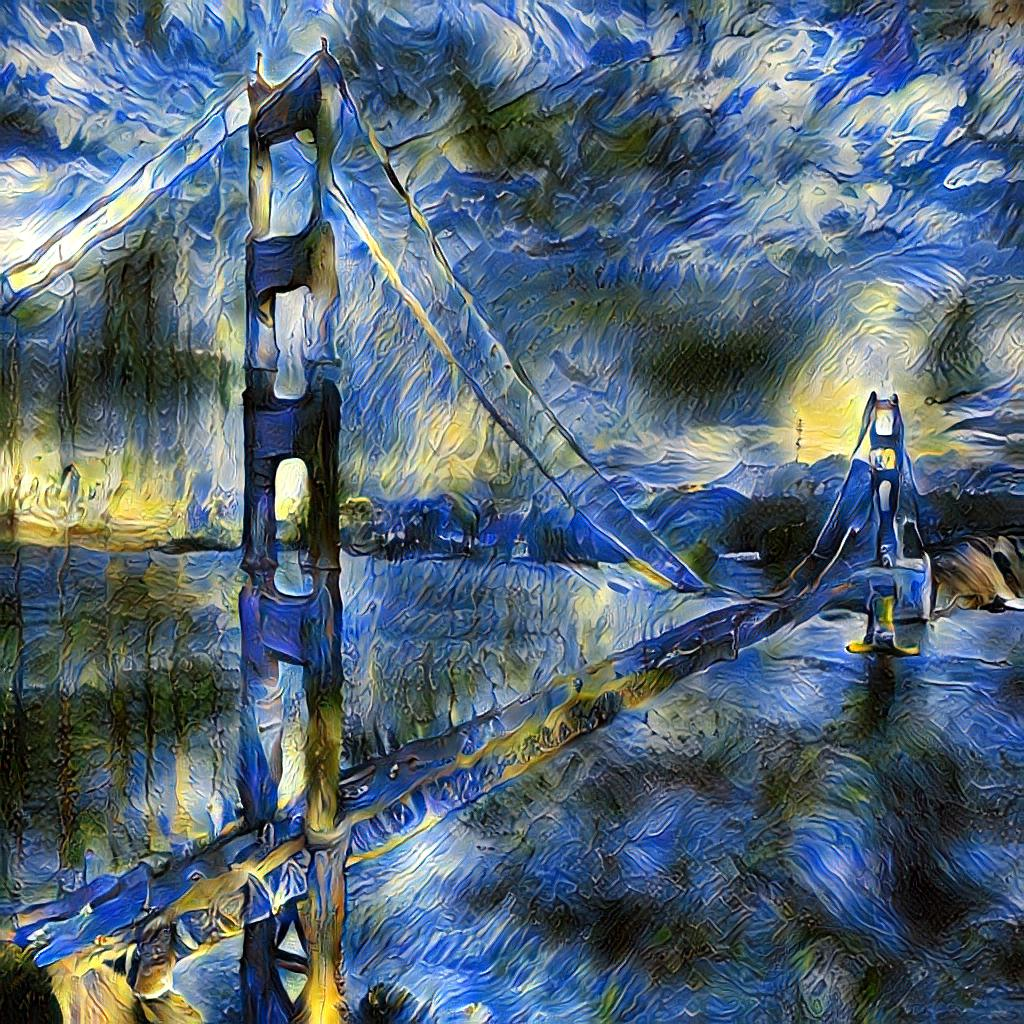
\includegraphics[width=\linewidth]{transfer_examples/transfer_bridge_starry_08_ref.jpg} % theirs reconstruction num.1	
	\end{subfigure}
	\begin{subfigure}[b]{0.225\linewidth}
		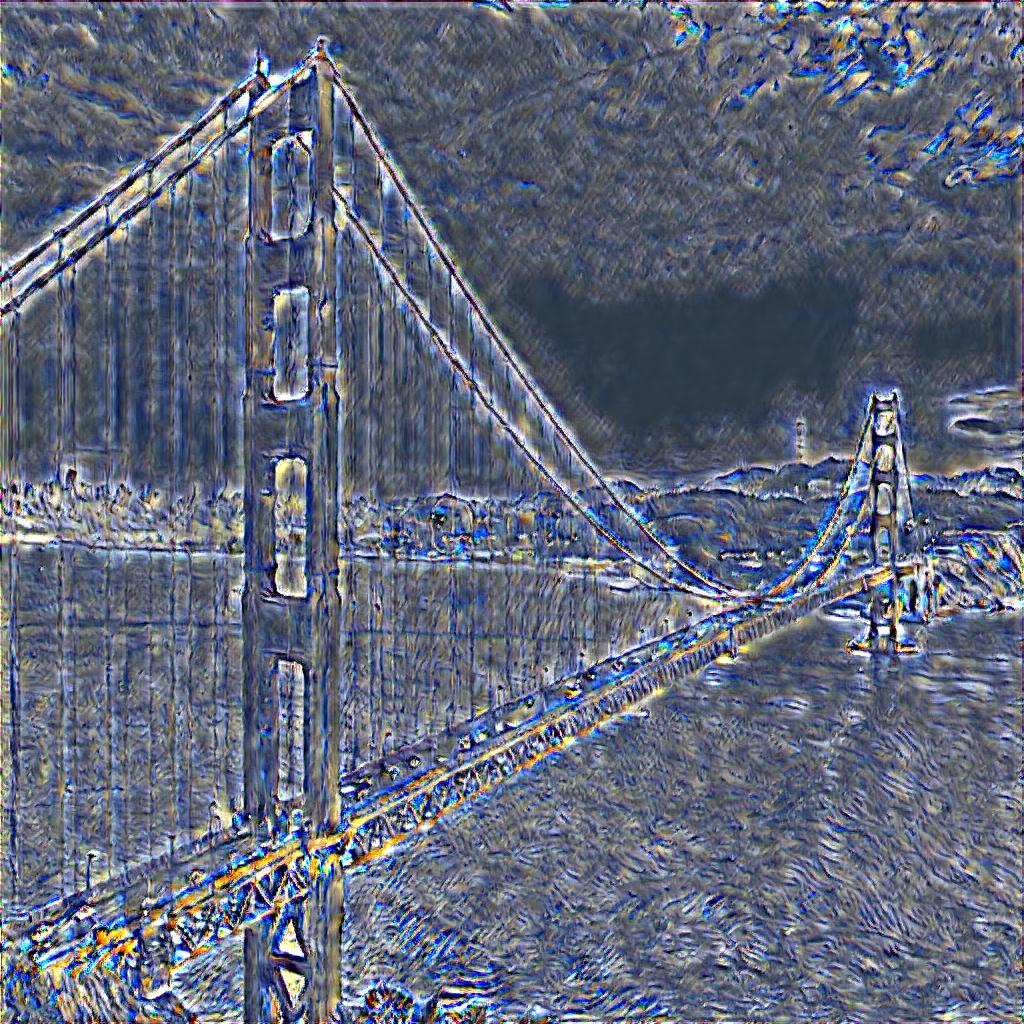
\includegraphics[width=\linewidth]{transfer_examples/transfer_bridge_starry_08_our.jpg} % ours reconstruction num.1	
	\end{subfigure}
	% second line
	\centering
	\begin{subfigure}[b]{0.225\linewidth}
		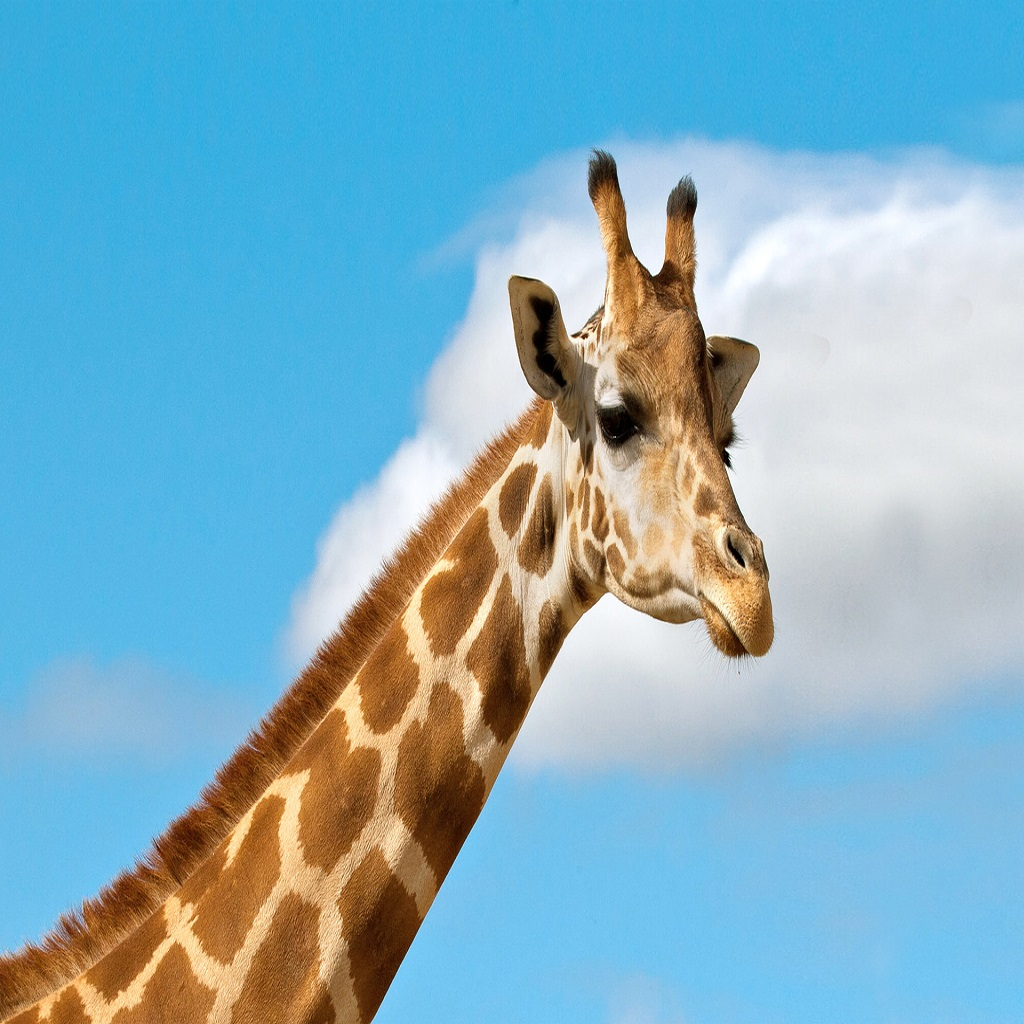
\includegraphics[width=\linewidth]{giraffe_sq.jpg} %style img num.2
	\end{subfigure}
	\begin{subfigure}[b]{0.225\linewidth}
		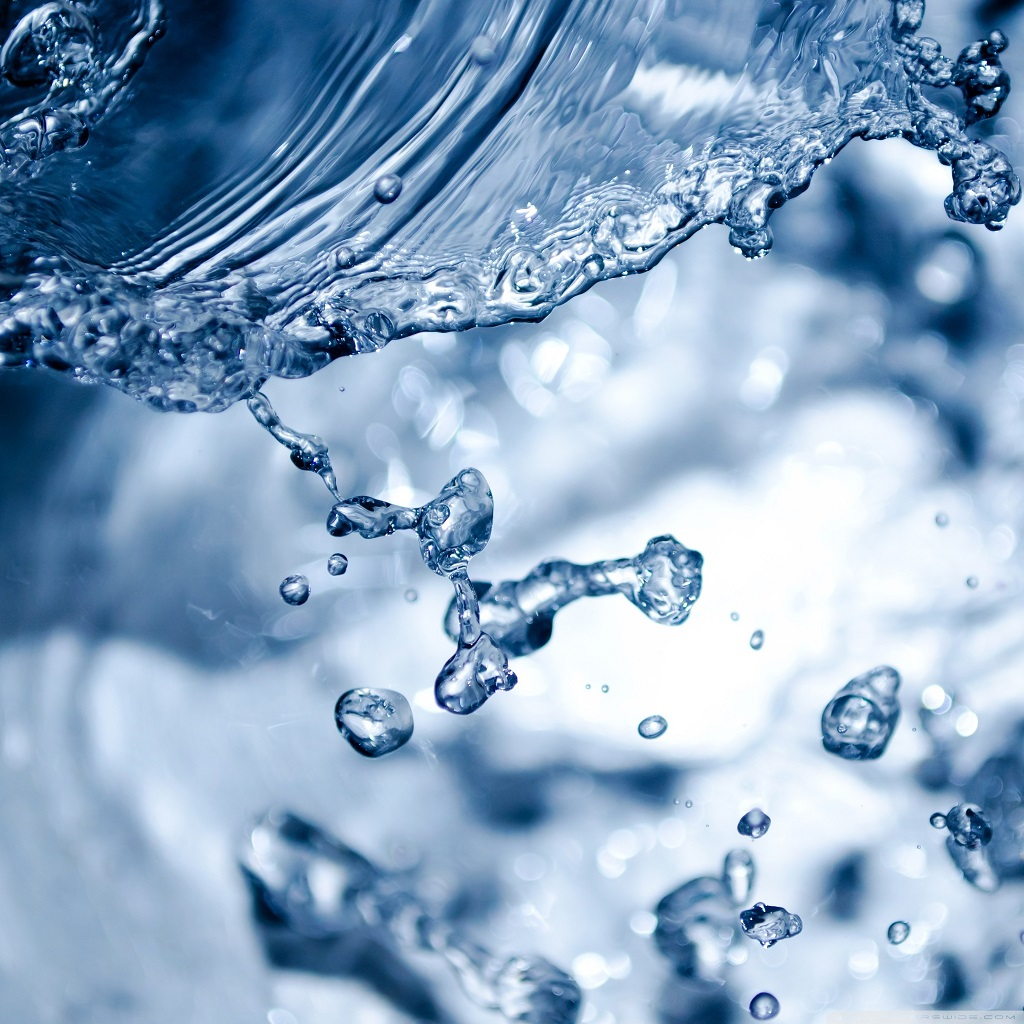
\includegraphics[width=\linewidth]{st1_sq.jpg} % content img num.2
	\end{subfigure}
	\begin{subfigure}[b]{0.225\linewidth}
		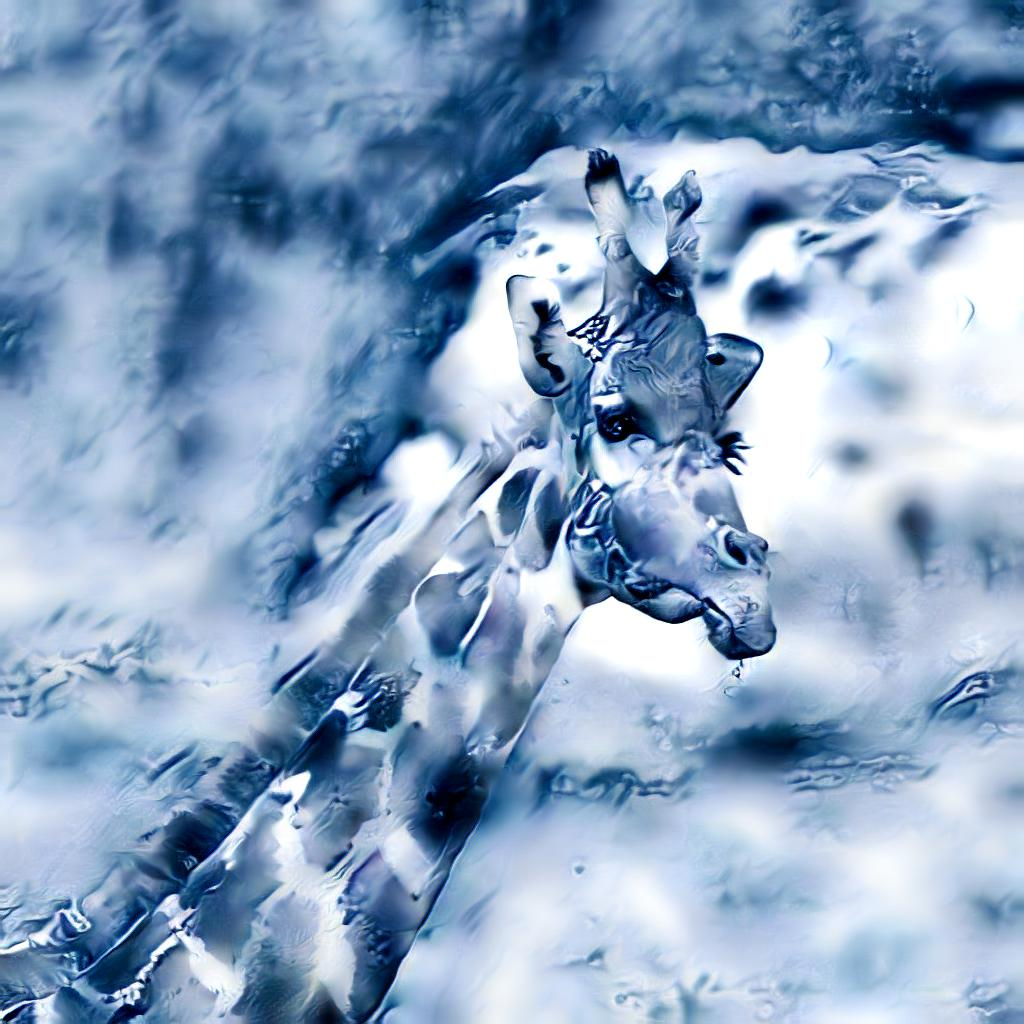
\includegraphics[width=\linewidth]{transfer_examples/transfer_giraffe_st1_08_ref.jpg} % theirs reconstruction num.2
	\end{subfigure}
	\begin{subfigure}[b]{0.225\linewidth}
		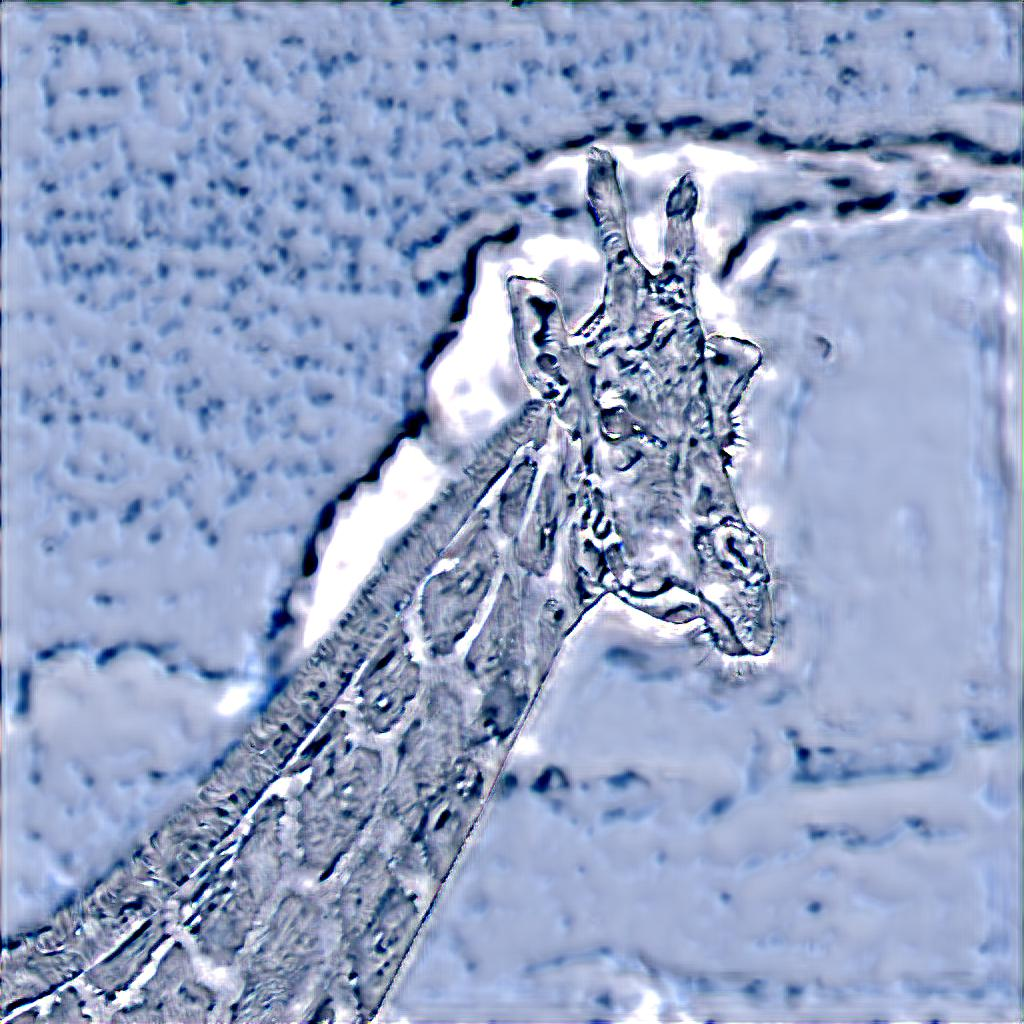
\includegraphics[width=\linewidth]{transfer_examples/transfer_giraffe_st1_08_our.jpg} % ours reconstruction num.2
	\end{subfigure}
	% third line
	\centering
	\begin{subfigure}[b]{0.225\linewidth}
		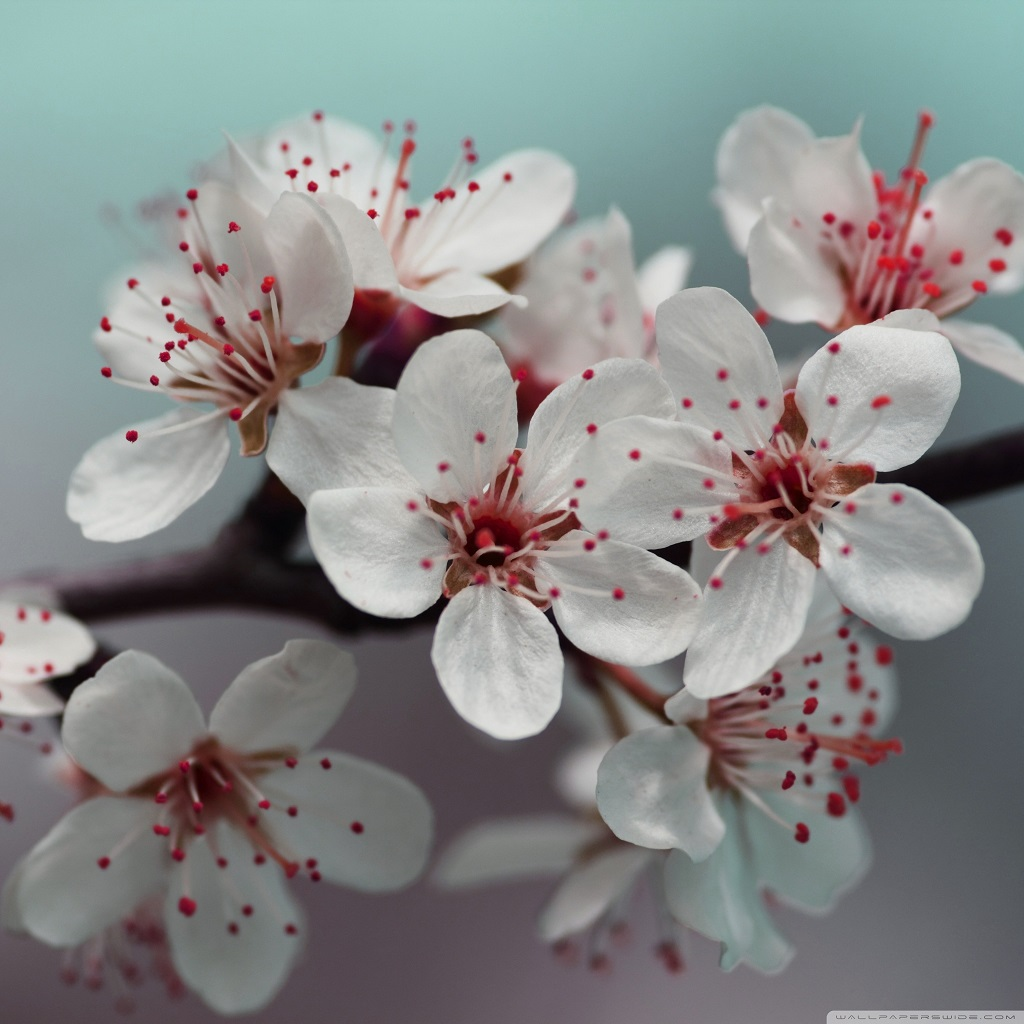
\includegraphics[width=\linewidth]{in1_sq.jpg} %style img num.3
	\end{subfigure}
	\begin{subfigure}[b]{0.225\linewidth}
		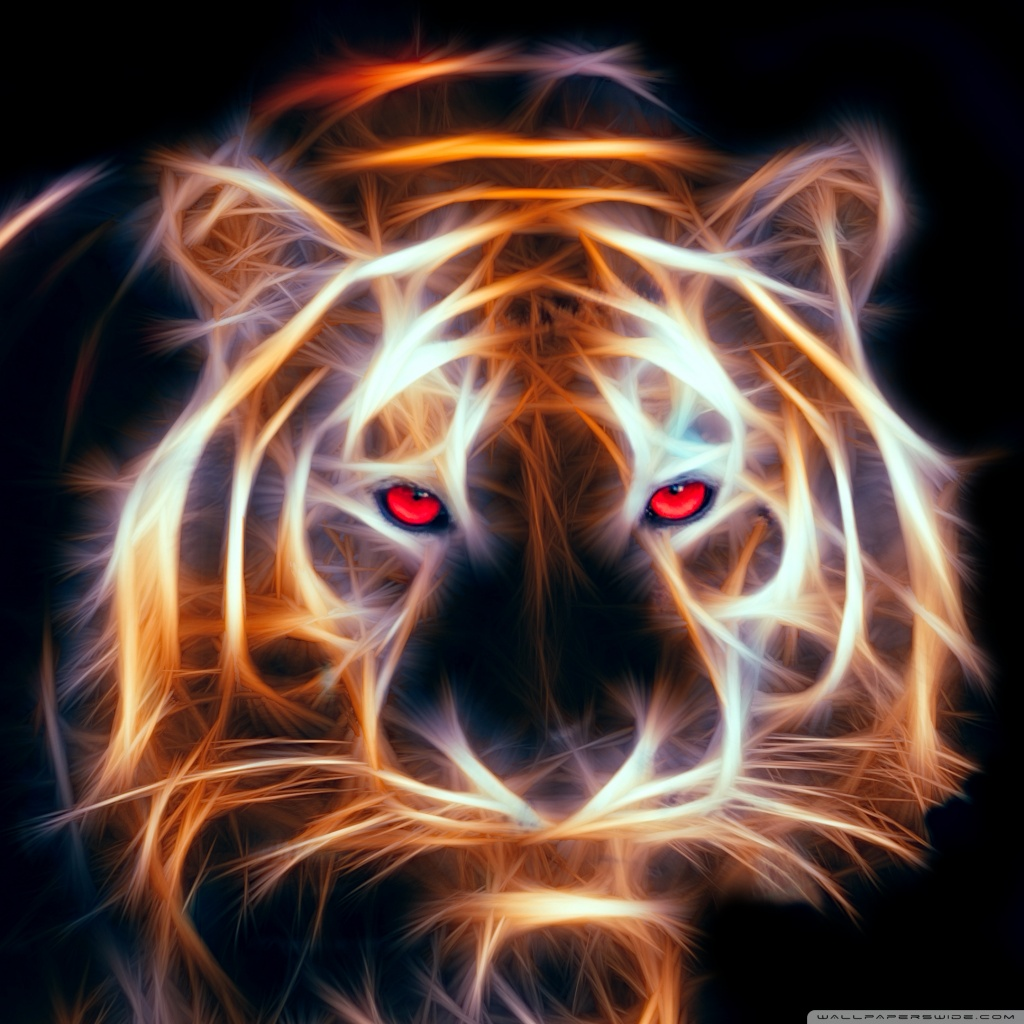
\includegraphics[width=\linewidth]{tiger_sq.jpg} % content img num.3
	\end{subfigure}
	\begin{subfigure}[b]{0.225\linewidth}
		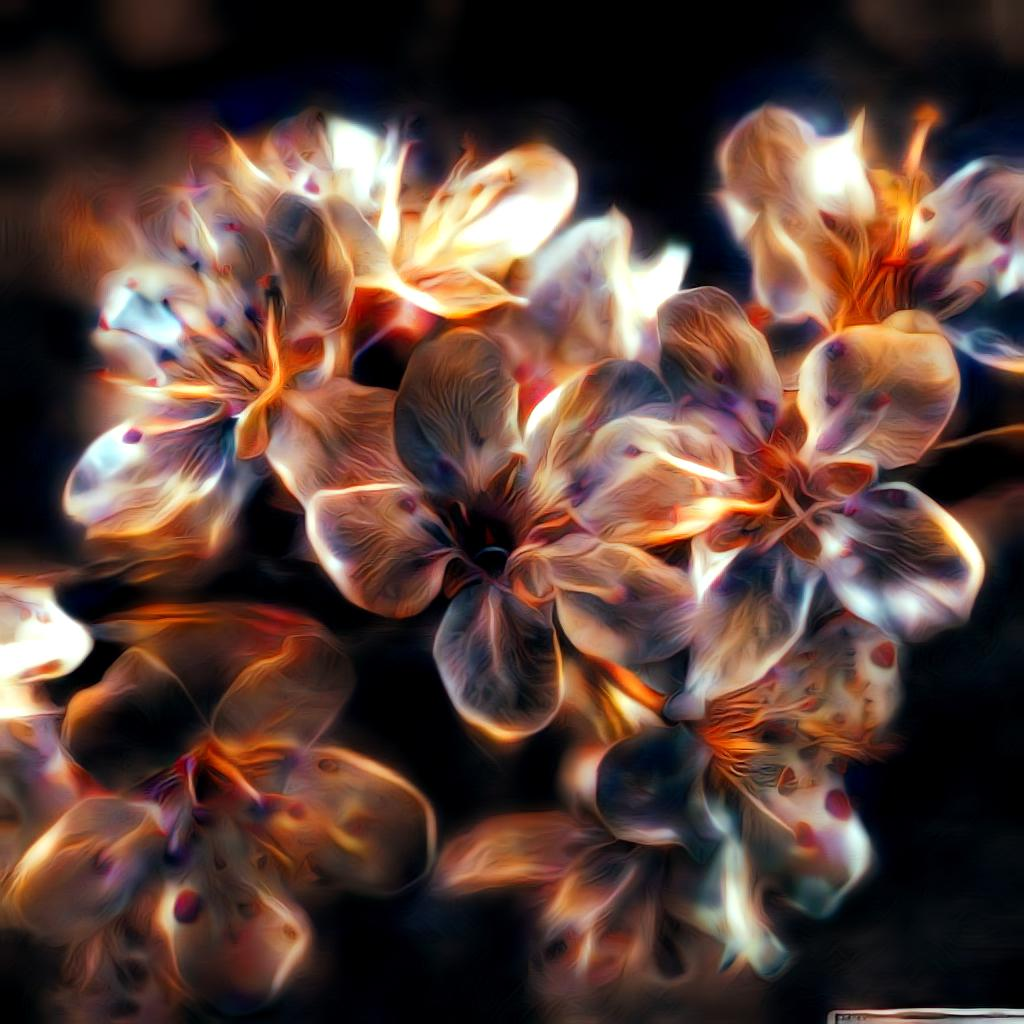
\includegraphics[width=\linewidth]{transfer_examples/transfer_in1_tiger_08_ref.jpg} % theirs reconstruction num.3
	\end{subfigure}
	\begin{subfigure}[b]{0.225\linewidth}
		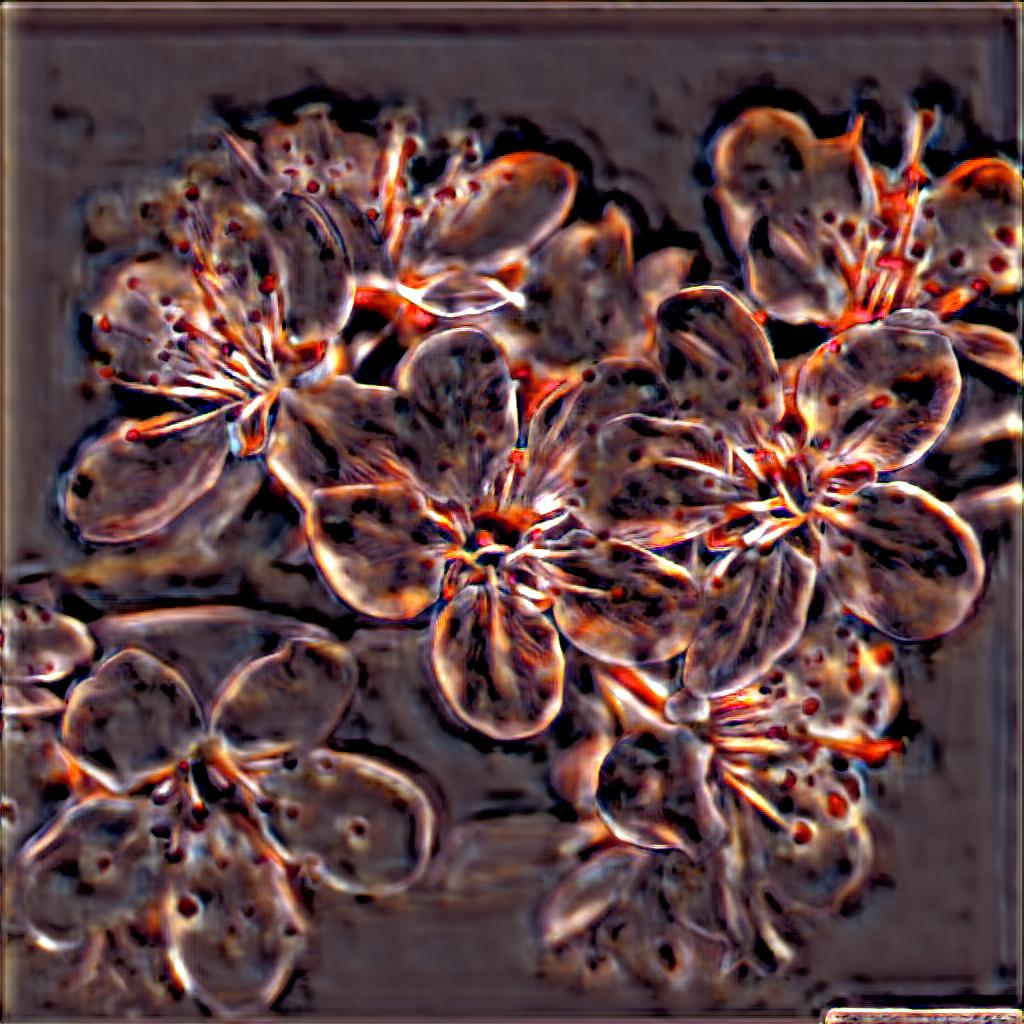
\includegraphics[width=\linewidth]{transfer_examples/transfer_in1_tiger_08_our.jpg} % ours reconstruction num.3
	\end{subfigure}
	% fourth line
	\centering
	\begin{subfigure}[b]{0.225\linewidth}
		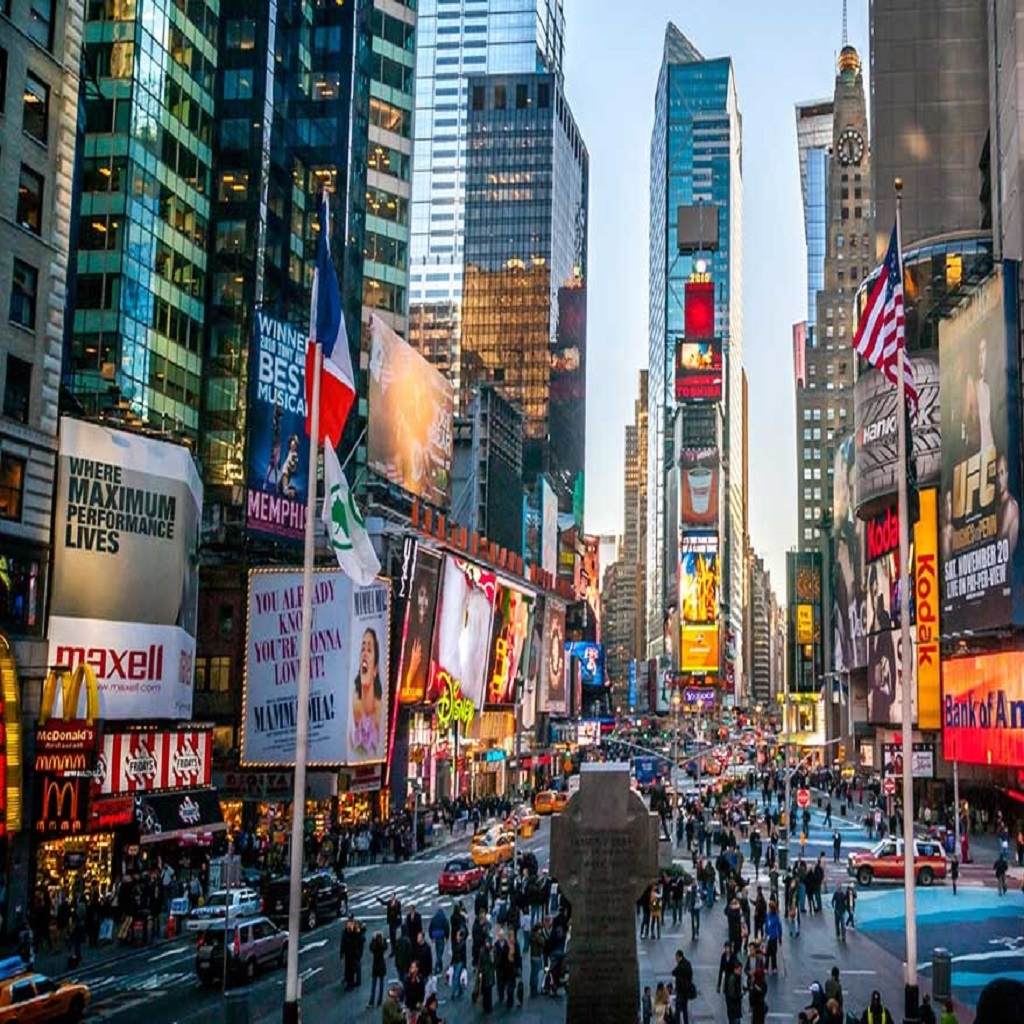
\includegraphics[width=\linewidth]{nyc_sq.jpg} %style img num.4
	\end{subfigure}
	\begin{subfigure}[b]{0.225\linewidth}
		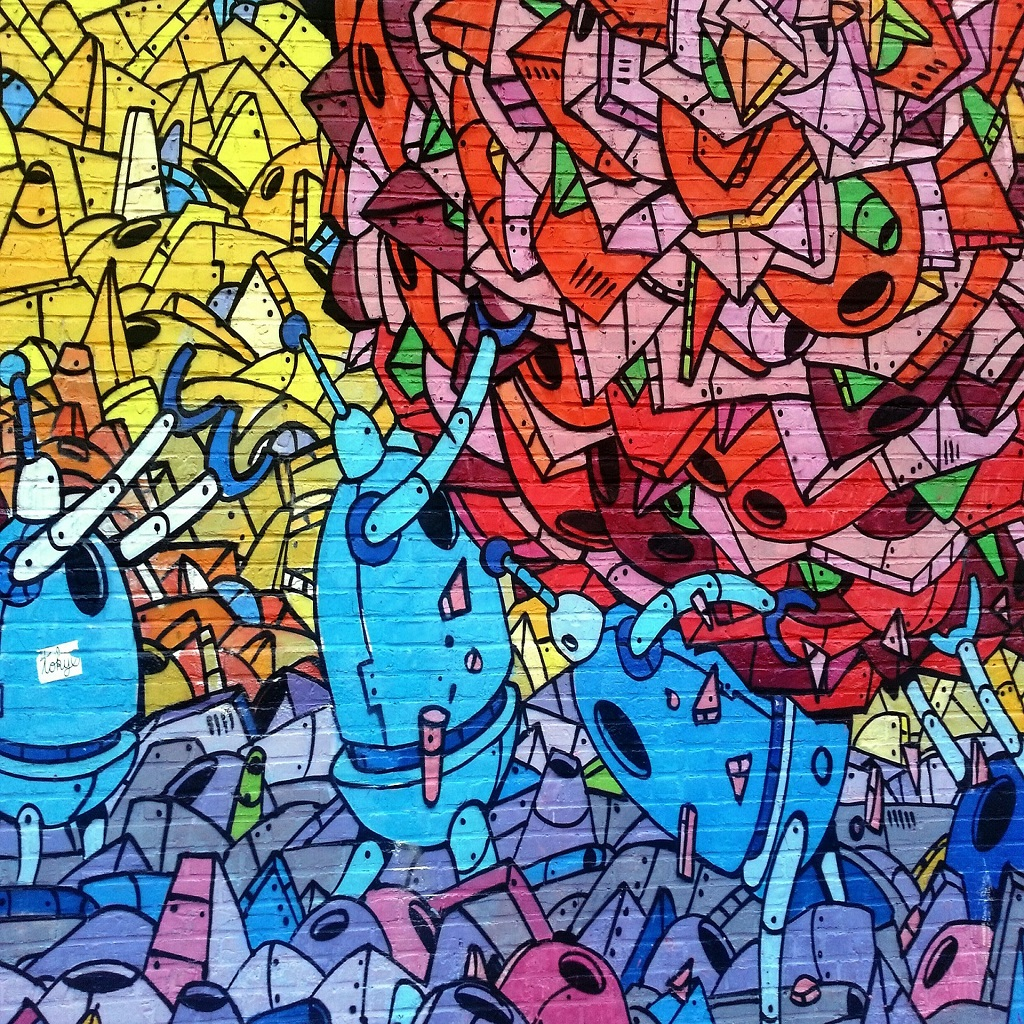
\includegraphics[width=\linewidth]{graffiti_sq.jpg} % content img num.4
	\end{subfigure}
	\begin{subfigure}[b]{0.225\linewidth}
		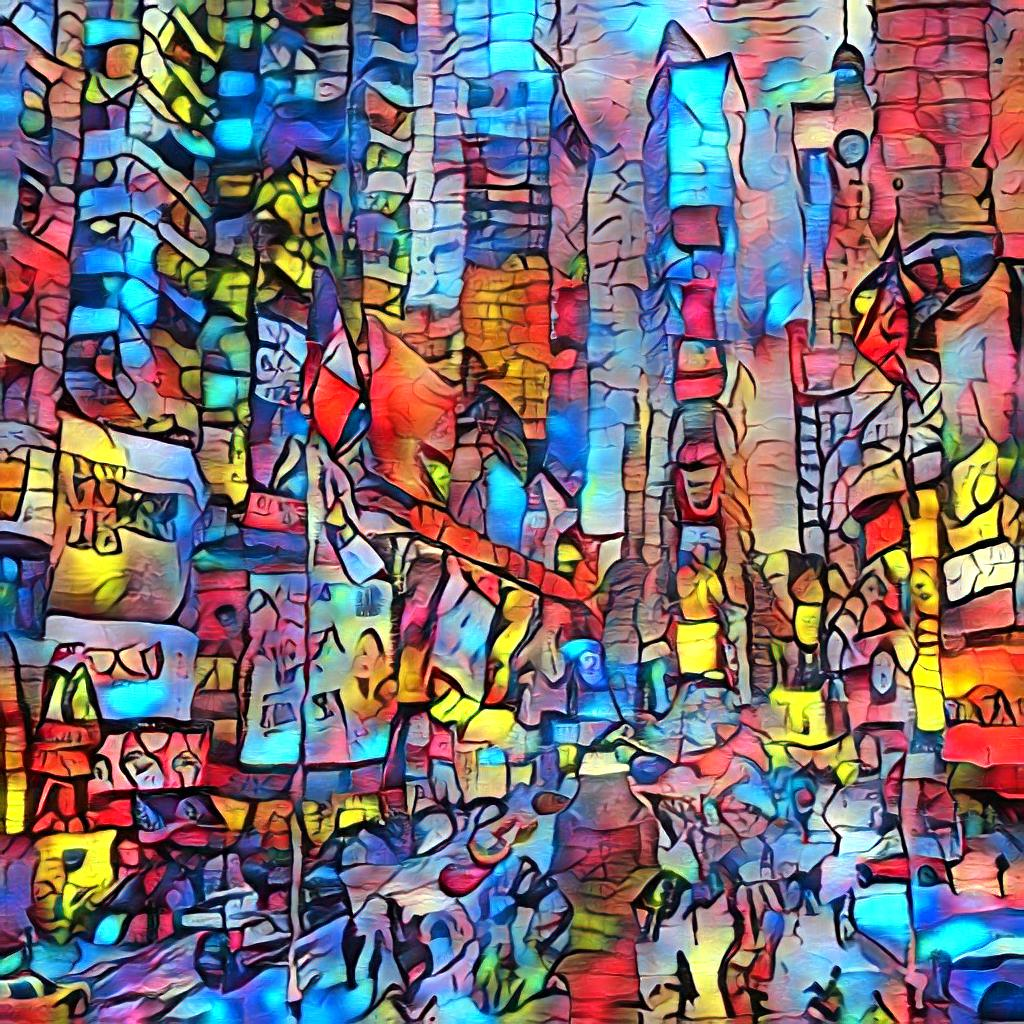
\includegraphics[width=\linewidth]{transfer_examples/transfer_nyc_graffiti_08_ref.jpg} % theirs reconstruction num.4
	\end{subfigure}
	\begin{subfigure}[b]{0.225\linewidth}
		\includegraphics[width=\linewidth]{transfer_examples/transfer_nyc_graffiti_08_our.jpg} % ours reconstruction num.4
	\end{subfigure}
	% fifth line
	\centering
	\begin{subfigure}[b]{0.225\linewidth}
		\includegraphics[width=\linewidth]{room_sq.jpg} %style img num.5
		\caption{Content}
	\end{subfigure}
	\begin{subfigure}[b]{0.225\linewidth}
		\includegraphics[width=\linewidth]{st2_sq.jpg} % content img num.5
		\caption{Style}
	\end{subfigure}
	\begin{subfigure}[b]{0.225\linewidth}
		\includegraphics[width=\linewidth]{transfer_examples/transfer_room_paint_08_ref.jpg} % theirs reconstruction num.5
		\caption{Reference Models}
	\end{subfigure}
	\begin{subfigure}[b]{0.225\linewidth}
		\includegraphics[width=\linewidth]{transfer_examples/transfer_room_paint_08_our.jpg} % ours reconstruction num.5
		\caption{Our Models}
	\end{subfigure}
	\caption{Results from different style transfer methods using style weight $\alpha=0.5$}
	\label{fig:style_transfer}
\end{figure}
%%%%%%%%%%%%%%%%%%%%%%%%%%%%
%%%%%%%%%%%%%%%%%%%%%%%%%%%%
% Boost %
%%%%%%%%%%%%%%%%%%%%%%%%%%%%
%%%%%%%%%%%%%%%%%%%%%%%%%%%%
\subsubsection{Stylization boosting}
\begin{figure}[H]
	% first line
	\centering
	\begin{subfigure}[b]{0.4\linewidth}
		\includegraphics[width=\linewidth]{car.jpg} %style img num.1
		\caption{Content}
	\end{subfigure}
	\begin{subfigure}[b]{0.4\linewidth}
		\includegraphics[width=\linewidth]{car.jpg} % content img num.1
		\caption{Style}
	\end{subfigure}
	%second line
	\begin{subfigure}[b]{0.4\linewidth}
		\includegraphics[width=\linewidth]{car.jpg} % regular UST num.1
		\caption{Regular UST}
	\end{subfigure}
	\begin{subfigure}[b]{0.4\linewidth}
		\includegraphics[width=\linewidth]{car.jpg} % UST+boost num.1
		\caption{Boost UST}
	\end{subfigure}
	\centering
	\begin{subfigure}[b]{0.4\linewidth}
		\includegraphics[width=\linewidth]{car.jpg} %style img num.1
		\caption{Content}
	\end{subfigure}
	\begin{subfigure}[b]{0.4\linewidth}
		\includegraphics[width=\linewidth]{car.jpg} % content img num.1
		\caption{Style}
	\end{subfigure}
	%second line
	\begin{subfigure}[b]{0.4\linewidth}
		\includegraphics[width=\linewidth]{car.jpg} % regular UST num.1
		\caption{Regular UST}
	\end{subfigure}
	\begin{subfigure}[b]{0.4\linewidth}
		\includegraphics[width=\linewidth]{car.jpg} % UST+boost num.1
		\caption{Boost UST}
	\end{subfigure}
	\caption{Boosting results comparing to original UST \cite{bib11}.}
	\label{fig:Boost}
\end{figure}
%%%%%%%%%%%%%%%%%%%%%%%% Merge  %%%%%%%%%%%%%%%%%%%%%%
\subsubsection{Two styles merging methods}
\begin{figure}[H]
	% first line
	\centering
	\begin{subfigure}[b]{0.13\linewidth}
		\includegraphics[width=\linewidth]{car.jpg} %style img num.1
	\end{subfigure}
	\begin{subfigure}[b]{0.13\linewidth}
		\includegraphics[width=\linewidth]{car.jpg} % style2 img num.1
	\end{subfigure}
	\begin{subfigure}[b]{0.13\linewidth}
		\includegraphics[width=\linewidth]{car.jpg} % content img num.1
	\end{subfigure}
	\begin{subfigure}[b]{0.13\linewidth}
		\includegraphics[width=\linewidth]{car.jpg} % orig merge num.1
	\end{subfigure}
	\begin{subfigure}[b]{0.13\linewidth}
		\includegraphics[width=\linewidth]{car.jpg} % merge1 num.1
	\end{subfigure}
	\begin{subfigure}[b]{0.13\linewidth}
		\includegraphics[width=\linewidth]{car.jpg} % merge2 num.1
	\end{subfigure}
	\begin{subfigure}[b]{0.13\linewidth}
		\includegraphics[width=\linewidth]{car.jpg} % merge3 num.1
	\end{subfigure}
	% second line
	\centering
	\begin{subfigure}[b]{0.13\linewidth}
		\includegraphics[width=\linewidth]{car.jpg} %style img num.2
	\end{subfigure}
	\begin{subfigure}[b]{0.13\linewidth}
		\includegraphics[width=\linewidth]{car.jpg} % style2 img num.2
	\end{subfigure}
	\begin{subfigure}[b]{0.13\linewidth}
		\includegraphics[width=\linewidth]{car.jpg} % content img num.2
	\end{subfigure}
	\begin{subfigure}[b]{0.13\linewidth}
		\includegraphics[width=\linewidth]{car.jpg} % orig merge num.2
	\end{subfigure}
	\begin{subfigure}[b]{0.13\linewidth}
		\includegraphics[width=\linewidth]{car.jpg} % merge1 num.2
	\end{subfigure}
	\begin{subfigure}[b]{0.13\linewidth}
		\includegraphics[width=\linewidth]{car.jpg} % merge2 num.2
	\end{subfigure}
	\begin{subfigure}[b]{0.13\linewidth}
		\includegraphics[width=\linewidth]{car.jpg} % merge3 num.2
	\end{subfigure}
	% third line
	\centering
	\begin{subfigure}[b]{0.13\linewidth}
		\includegraphics[width=\linewidth]{car.jpg} %style img num.3
		\caption{$1_{st}$ \\ Style}
	\end{subfigure}
	\begin{subfigure}[b]{0.13\linewidth}
		\includegraphics[width=\linewidth]{car.jpg} %style2 img num.3
		\caption{$2_{nd}$ \\ Style}
	\end{subfigure}
	\begin{subfigure}[b]{0.13\linewidth}
		\includegraphics[width=\linewidth]{car.jpg} % content img num.3
		\caption{Content \\ image}
	\end{subfigure}
	\begin{subfigure}[b]{0.13\linewidth}
		\includegraphics[width=\linewidth]{car.jpg} % orig merge num.3
		\caption{Li et al. \cite{bib11}}
	\end{subfigure}
	\begin{subfigure}[b]{0.13\linewidth}
		\includegraphics[width=\linewidth]{car.jpg} % merge1 num.3
		\caption{$1_{st}$ method}
	\end{subfigure}
	\begin{subfigure}[b]{0.13\linewidth}
		\includegraphics[width=\linewidth]{car.jpg} % merge2 num.3
		\caption{$2_{nd}$ method}
	\end{subfigure}
	\begin{subfigure}[b]{0.13\linewidth}
		\includegraphics[width=\linewidth]{car.jpg} % merge3 num.3
		\caption{$3_{rd}$ method}
	\end{subfigure}
		\caption{Results using different stylization methods. (d) is the original merge method as in \cite{bib11}, (e) is Level Merge, (f) is Channel Merge and (g) is Interpolate-Style Merge.}
		\label{fig:Merge}
\end{figure}
%%%%%%%%%%%%%%%%%%%%%%%%%%%%
add more text here
%%%%%%%%%%%%%%%%%%%%%%%% Texture synthesis  %%%%%%%%%%%%%%%%%%%%%%
\subsubsection{Texture synthesis}
We demonstrate the effectiveness of our method for universal style transfer by showing its application to universal texture synthesis. In figure ~\ref{fig:texture} we visualize the whitened features and
synthesized textures via simple feature coloring.
One option to produce texture image is simply setting the content image as a random noise image (e.g., Gaussian noise). Another option to get synthesized texture in our stylization framework is to directly initialize the content features to be white noise as proposed by Li et al. \cite{bib11}. Both approaches achieve similar results.
The evaluation criterion for the quality of the synthesized texture is usually human inspection and textures are successfully synthesized if a human observer cannot tell the original texture from a synthesized one.
\begin{figure}[H]
	% first line
	\centering
	\begin{subfigure}[b]{0.4\linewidth}
		\includegraphics[width=\linewidth]{car.jpg} %texture img num.1
	\end{subfigure}
	\begin{subfigure}[b]{0.4\linewidth}
		\includegraphics[width=\linewidth]{car.jpg} % content img num.1
	\end{subfigure}
	% second line
	\centering
	\begin{subfigure}[b]{0.4\linewidth}
		\includegraphics[width=\linewidth]{car.jpg} %content img num.3
		\caption{Style}
	\end{subfigure}
	\begin{subfigure}[b]{0.4\linewidth}
		\includegraphics[width=\linewidth]{car.jpg} % stylization img num.3
		\caption{Our UST}
	\end{subfigure}
	\caption{Synthesized results using our UST implementation.}
	\label{fig:texture}
\end{figure}